\documentclass[11pt,review,authoryear]{elsarticle}
\RequirePackage{amsthm,amsmath,amsfonts,amssymb}
\RequirePackage[colorlinks,linkcolor=cyan,citecolor=red,urlcolor=magenta]{hyperref}
\RequirePackage{fix-cm}

\usepackage[table,xcdraw]{xcolor}
\usepackage{arydshln}
\usepackage{color,soul}
\usepackage{accents,float,graphicx,subfig,multirow,dcolumn,booktabs,lscape}
\usepackage{comment}
\usepackage[letterpaper,margin=0.9in]{geometry}
\usepackage[ruled,linesnumbered]{algorithm2e}
\usepackage[font=normal]{caption}
\usepackage[title]{appendix}

%thick cdot
\makeatletter
\newcommand*\bigcdot{\mathpalette\bigcdot@{.5}}
\newcommand*\bigcdot@[2]{\mathbin{\vcenter{\hbox{\scalebox{#2}{$\m@th#1\bullet$}}}}}
\makeatother

\newcommand{\size}[2]{{\fontsize{#1}{0}\selectfont#2}}
\newenvironment{sizepar}[2]
 {\par\fontsize{#1}{#2}\selectfont}
 {\par}

\SetAlFnt{\small}

\pagestyle{myheadings}

%eqn, def numbering
\numberwithin{equation}{section}

\theoremstyle{definition}
\newtheorem{definition}{\protect\definitionname}
\providecommand{\definitionname}{Definition}
\numberwithin{definition}{section}

\theoremstyle{plain}
\newtheorem{lemma}{\protect\lemmaname}
\providecommand{\lemmaname}{Lemma}
\numberwithin{lemma}{section}

\theoremstyle{plain}
\newtheorem{theorem}{\protect\theoremname}
\providecommand{\theoremname}{Theorem}
\numberwithin{theorem}{section}

\newcommand{\appendixpagenumbering}{
  \break
  \pagenumbering{arabic}
  \renewcommand{\thepage}{\thesection-\arabic{page}}
}

% highlighting
\newcommand{\hlgreen}[2][green]{{\sethlcolor{#1}\hl{#2}}}
\newcommand{\hlning}[2][orange]{{\sethlcolor{#1}\hl{#2}}}

\newcommand{\ind}{\perp\!\!\!\!\perp}
\newcommand{\ts}{\rlap{$^{***}$}}
\newcommand{\ds}{\rlap{$^{**}$}}
\newcommand{\s}{\rlap{$^{*}$}}

\def\spacingset#1{\renewcommand{\baselinestretch}{#1}\small\normalsize}\spacingset{1}

\newcolumntype{.}{D{.}{.}{-1}}

% path for figures
\graphicspath{{figures/}}

% Remove irritating PDFLaTeX warnings
%\pdfminorversion=6
\pdfminorversion=7
\pdfsuppresswarningpagegroup=1


%%%%%%%%%%%%%%%%%%%%%%%%%%%
%%%%%%%%%%%%%%%%%%%%%%%%%%%
%%%%%%%%%%%%%%%%%%%%%%%%%%%

\begin{document}

\title{Solar: stable and ultrafast variable selection for high dimensional and large-scale data}

\author{Ning Xu\corref{cor1}}
\ead{n.xu@sydney.edu.au}
\address{School of Economics, University of Sydney, Australia}

\author{Timothy C.G. Fisher\corref{cor2}}
\ead{tim.fisher@sydney.edu.au}
\address{School of Economics, University of Sydney, Australia}

\author{Jian Hong}
\ead{jian.hong@sydney.edu.au}
\address{School of Economics, University of Sydney, Australia}


\cortext[cor1]{Principal corresponding author.}
\cortext[cor2]{Corresponding author.}

\begin{abstract}
  %
  We propose a new algorithm for variable selection in high-dimensional, large-scale data, called \emph{subsample-ordered least-angle regression (solar)} and a coordinate-descent generalization \emph{(solar-cd)}. By averaging and re-ordering lasso paths using the $L_0$ norm, solar can easily be modified to replace many lasso variants. Solar alleviates several high-dimensional issues with lasso, such as the strong/safe rules, variable screening, and subsampling variable selection. Using examples, simulations, and real-world data, we illustrate: (i) with the same computation load, solar yields substantial improvements over lasso in terms of the sparsity (37-64\% reduction in false variable selection), stability, and accuracy of variable selection; (ii) compared with the lasso strong/safe rule and variable screening, solar largely rectifies incorrect variable purging and sparsity loss with complicated dependence structures and harsh settings of the irrepresentable condition; (iii) solar supplemented with the hold-out average test (an adaptation of data-splitting hypothesis testing) dramatically improves the efficiency and accuracy of post-selection inference; (iv) replacing lasso with solar in subsampling variable selection (e.g., the bootstrap lasso or stability selection) produces a novel \emph{multi-layer} variable ranking scheme, resulting in improvements in selection sparsity, ranking accuracy, and huge computation load reductions (a saving of at least 96\% in runtime, substantially beyond the theoretical maximum speedup for parallelizing the lasso-type algorithm.) Using a Python interface and an Intel MKL Fortran/C++ compiler, we provide a parallel computing package for solar (\texttt{solarpy}) in the supplementary file and at the dedicated \href{https://github.com/isaac2math/solarpy}{Github page}.
  %
\end{abstract}

\begin{keyword}
Sparsity, complicated dependence structure, irrepresentable condition, lasso rule, bolasso, subsampling variable selection, variable screening.
\end{keyword}

\maketitle

\spacingset{1.4}

%%%%%%%%%%%%%%%%%%%%%%%%%%%%%%%
%%%%%%%% INTRODUCTION  %%%%%%%%
%%%%%%%%%%%%%%%%%%%%%%%%%%%%%%%

\pagenumbering{arabic}

\section{Introduction}

In the last decade, lasso-related algorithms have been widely applied to high dimensional, large-scale applications \citep{efronall04, friedman2007pathwise, friedman2010regularization}. Various improvements have been proposed for lasso to address known issues of computation speed, selection sparsity, stability, and accuracy \citep{weisberg04, lim2016estimation}. Subsampling variable selection (e.g., \citet{bach2008bolasso, meinshausen2010stability}) has emerged as one of the most effective improvements to the variable-selection accuracy and stability of lasso. Given that optimization of the lasso-type tuning parameter is often combined with cross validation (CV), computing CV-lasso on each bootstrap subsample sharply increases the computation load, making any subsampling-based lasso variants less attractive in large-scale applications such as computer vision and natural language processing (where $p$ may be in the millions and data in the GBs) \citep{xu2012asymptotic}. Thus, in a world of ever-expanding data dimensionality, it is critical that improvements in variable selection are accompanied with significant computation load reductions.

Post-lasso selection rules (e.g., the `safe rule' \citep{ghaoui2010safe} and the `strong rule' \citep{tibshirani2012strong}) are capable of improving lasso without exponentially increasing the computation runtime. However, the rules may falsely purge informative variables or propose repeated modifications \citep{wang2014safe, zeng2017efficient}. Alternatively, \citet{wasserman2009high}, \citet{meinshausen2009p} and \citet{barber2019knockoff} propose data splitting to conduct classical hypothesis tests after subsample selection. The original data are split into two: one part for variable selection, the other for testing. However, to improve test power, data-splitting must be repeated on each bootstrap sample, raising similar computational concerns as subsampling variable selection \citep{bach2008bolasso,meinshausen2010stability}. \citet{diciccio2020exact} also conclude that because data splitting reserves a portion of the data for variable selection, it reduces the degrees of freedom for testing on the remaining data, which may be a problem when the original sample size is limited. Lastly, \citet{fan2008sure} propose the variable screening algorithm, which ranks the absolute values of unconditional correlations between each covariate and the response variable, selecting only the top-ranked variables. However, \citet{fan2008sure} and \citet{barut2016conditional} (and Section~\ref{section:example} below) show that variable screening methods also suffer from invalid variable selection and purging when the dependence structure is complicated.

\subsection{Main results}

To address these issues, we propose a new algorithm for variable selection in high-dimensional, large-scale data, called \emph{subsample-ordered least-angle regression} (\emph{solar}), and a coordinate-descent generalization (\emph{solar-cd}). Because solar is based on averaging and re-ordering lasso paths via the $L_0$ norm, it is easily adaptable to many lasso variants. Solar alleviates the high-dimensional issues with lasso, such as the strong/safe rules, variable screening, and subsampling variable selection while having the same computation load as lasso.

Using simulations, examples, and real-world data, we demonstrate the following advantages of solar: (i) with the same computation load, solar yields substantial improvements over lasso in terms of the sparsity (37-64\% reduction in false variable selection), stability, and accuracy of variable selection; (ii) compared with the lasso strong/safe rule and variable screening, solar largely rectifies incorrect variable purging and sparsity loss in the presence of complicated dependence structures and harsh settings of the irrepresentable condition; (iii) solar supplemented with the hold-out average test (an adaptation of data-splitting hypothesis testing) substantially improves the efficiency and accuracy of post-selection inference; (iv) replacing lasso with solar in subsampling variable selection (e.g., the bootstrap lasso or stability selection) produces a novel \emph{multi-layer} variable ranking scheme that brings improvements in selection sparsity, ranking accuracy, and computation resources (a saving of at least 96\% in runtime, substantially beyond the theoretical maximum speedup for parallelizing the lasso-type algorithm.). Using a Python interface and an Intel MKL Fortran/C++ compiler, we provide a parallel computing package for solar (solarpy) in the supplementary file and at the dedicated \href{https://github.com/isaac2math/solarpy}{Github page}.

The paper is organized as follows. In section~\ref{section:algo}, we introduce solar and its coordinate descent generalization. In section~\ref{section:adv} and \ref{section:comp}, we  use examples and simulations to demonstrate solar's improvements over lasso, the strong/safe rules, variable screening, forward regression and the lasso-related, subsampling variable selection. In section~\ref{section:application}, we use real-world data that exhibits complicated dependency structures to show that the improvements from solar are feasible, while lasso and elastic net lose sparsity.

%%%%%%%%%%%%%%%%%%%%%%%
%%%%%% SECTION 2 %%%%%%
%%%%%%%%%%%%%%%%%%%%%%%

\section{Solar algorithm \label{section:algo}}

The solar improvements over lasso and lasso-related subsampling variable selection are due to a reallocation of computation. Lasso and its variants allocate most of the computation to optimizing the shrinkage parameter $t$ and $\lambda$ using cross-validation. By contrast, with the same computation load, solar allocates computation to stabilizing the solution path, which is key to the variable selection procedure. \citet[Theorem~2]{zhang09} implies that the earlier a variable enters the solution path, the more likely it is informative. As a result, a stable and accurate ordering of variables in the solution path may help identify informative variables. Since we focus on variable selection accuracy, the only relevant feature of the regression coefficients in the solution path is whether $\beta_i = 0$ at each stage. Thus, for least-angle regression and pathwise cooridinate descent, we reparametrize the lasso path via the $L_0$ norm.
%
\begin{definition}[$L_0$ solution path]
  %
  Define the \textbf{$L_0$ solution path} on $\left( Y, X \right)$ to be the order that least-angle regression includes variables across all stages. For example, if the least angle regression includes $\mathbf{x}_3$ at stage 1, $\mathbf{x}_2$ at stage 2 and $\mathbf{x}_1$ at stage 3, the corresponding $L_0$ path is the ordered set $\left\{ \left\{\mathbf{x}_3 \right\}, \left\{ \mathbf{x}_3, \mathbf{x}_2 \right\}, \left\{ \mathbf{x}_3, \mathbf{x}_2, \mathbf{x}_1 \right\} \right\}$.
  %
  \label{def:solution_path}
  %
\end{definition}

\subsection{Solar solved by least angle regression}

The solution path is the foundation of a $L_p$-penalized regression. To stabilize the regression performance in high-dimensional spaces, we first reduce the sensitivity of the solution path when $p > n$. The \emph{average $L_0$ solution path estimation} algorithm (summarized in Algorithm~\ref{algo:APE-lar} and illustrated in Figure~\ref{fig:q_demo}) accomplishes this task by estimating the \emph{average stage $\mathbf{x}_i$ enters the solution path} of least-angle regression.

\smallskip
\begin{algorithm}[h]

  \SetKwData{Left}{left}\SetKwData{This}{this}\SetKwData{Up}{up}
  \SetKwFunction{Union}{Union}\SetKwFunction{FindCompress}{FindCompress}
  \SetKwInOut{Input}{input}\SetKwInOut{Output}{output}

  \smallskip
  \Input{$\left( Y, X \right)$.}

  generate $K$ subsamples $\left\{ \left( Y^k, X^k \right) \right\}^{K}_{k=1}$ by randomly remove $1/K$ of observations in $\left( Y, X \right)$\;

  set $\widetilde{p} = \min\left\{ n_{\mathrm{sub}}, p \right\}$\;

  \For{ k := 1 to K, stepsize = 1 \nllabel{outer_averaging_start} }{

    run an unrestricted least-angle regression on $\left( Y^k, X^k \right)$ and record the order of variable inclusion at each stage\;
    \nllabel{inner_averaging_start}

    define $\widehat{q}^k = \mathbf{0} \in \mathbb{R}^p$\;

    $\forall i,l \in \mathbf{N}^+$, if $\mathbf{x}_i$ is included at stage $l$ and excluded at $l-1$, set $\widehat{q}^k_i= (\widetilde{p} + 1 - l) / \widetilde{p}$, where $\widehat{q}^k_i$ is the $i$\textsuperscript{th} entry of $\widehat{q}^k$\;
    \nllabel{inner_averaging_end}

    }

  $\widehat{q} := \frac{1}{K} \sum_{k=1}^{K} \widehat{q}^k$\; \nllabel{outer_averaging_end}

  \Return $\widehat{q}$

\caption{average $L_0$ path estimation via least angle regression \label{algo:APE-lar}}

\end{algorithm}

%%%%%%%%%%%%%%%%%%

\begin{figure}[h]
%
  \centering
%
  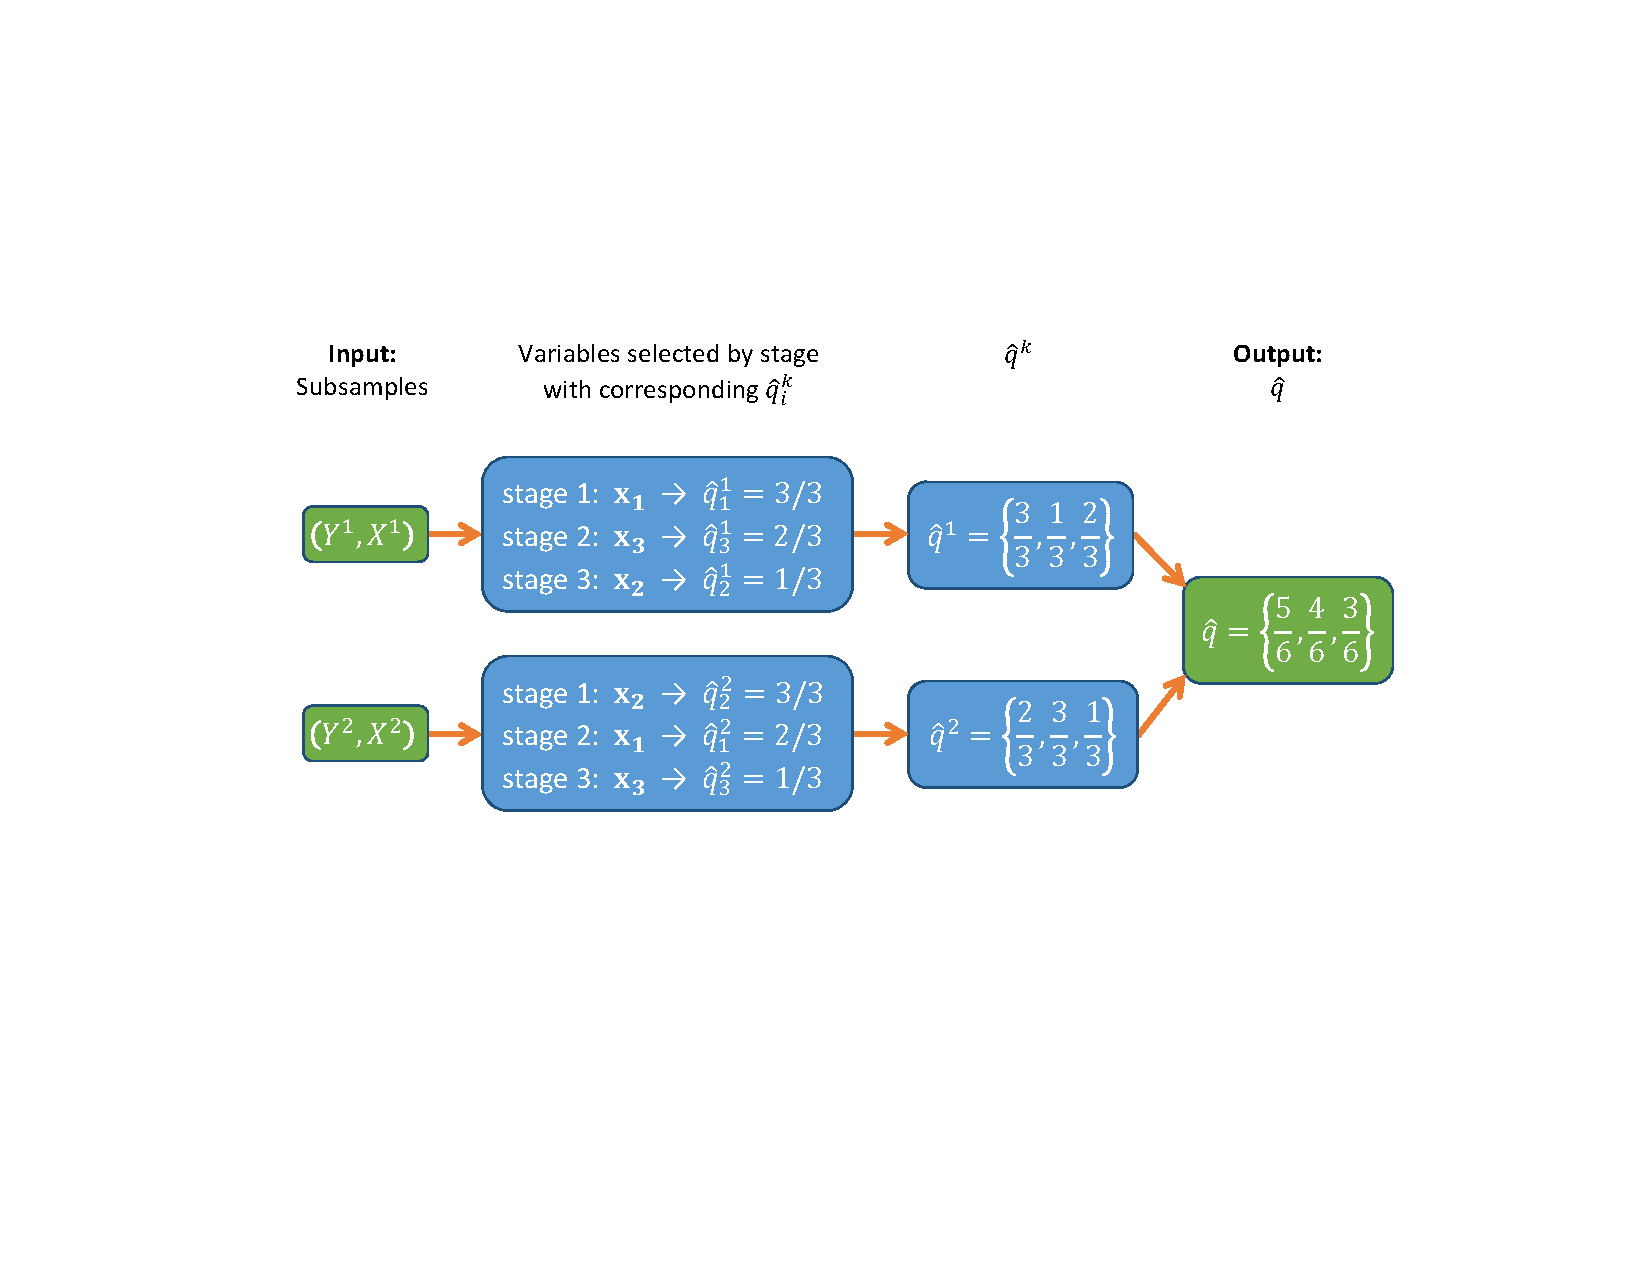
\includegraphics[width=0.66\paperwidth]{q_demo_1new.pdf}
%
  \caption{Computation of $\widehat{q}$ on 2 subsamples where $\left\{ \mathbf{x}_1, \mathbf{x}_2 \right\}$ are informative and $\mathbf{x}_3$ redundant.}
%
  \label{fig:q_demo}
%
\end{figure}

After subsampling, the second part of Algorithm~\ref{algo:APE-lar} (lines~\ref{inner_averaging_start}-\ref{inner_averaging_end}) computes $\widehat{q}^k$, which summarizes the order that least angle regression includes each $\mathbf{x}_i$ across all stages (as in the Figure~\ref{fig:q_demo} example). The unrestricted least-angle regression only ranks variables by the stage $\mathbf{x}_i$ enters the solution path. As shown in line~\ref{inner_averaging_end} of Algorithm~\ref{algo:APE-lar} and Figure~\ref{fig:q_demo}, variables included at earlier stages have larger corresponding $\widehat{q}^k_i$ values: the first variable included is assigned $1$, the last is assigned $1/\widetilde{p}$ and the dropped variables are assigned $0$ (which occurs only when $p > n$). Thus, by ranking (decreasingly) the $\mathbf{x}_i$ according to their corresponding $\widehat{q}^k_i$ values, we obtain the $L_0$ solution path. The \citet[Theorem 2]{zhang09} result implies that the variables with the largest $\widehat{q}^k_i$ values, on average, are more likely to be informative variables. The $\widehat{q}^k_i$ may be sensitive in high-dimensional spaces to multicollinearity, sampling randomness and noise. A consequence is that a redundant variable may be included at an early stage in some subsample $\left( Y^k, X^k \right)$. Hence, Algorithm~\ref{algo:APE-lar} reduces the impact of sensitivity in the $\widehat{q}^k_i$ values by computing $\widehat{q} := \frac{1}{K} \sum_{k=1}^{K} \widehat{q}^k$ and ranking the $\mathbf{x}_i$ (decreasingly) based on the corresponding value of $\widehat{q}_i$ (the $i$\textsuperscript{th} entry of $\widehat{q}$), to get the average $L_0$ solution path. The average $L_0$ solution path is formally defined as follows.
%
\begin{definition}[average $L_0$ solution path]
  %
  Define the \textbf{average $L_0$ solution path} of least-angle regression on $\left\{ \left( Y^k, X^k \right) \right\}_{k=1}^{K}$ to be the decreasing rank order of variables based on their corresponding $\widehat{q}_i$ values. For example, in Figure~\ref{fig:q_demo}, the $\widehat{q}_i$ values for $\mathbf{x}_1$, $\mathbf{x}_2$ and $\mathbf{x}_3$ are, respectively, $\widehat{q}_1 = 5/6$, $\widehat{q}_2 = 4/6$ and $\widehat{q}_3 = 3/6$. As a result, the average $L_0$ solution path can be represented as an ordered set $\left\{ \left\{ \mathbf{x}_1 \right\}, \left\{ \mathbf{x}_1, \mathbf{x}_2 \right\}, \left\{ \mathbf{x}_1, \mathbf{x}_2, \mathbf{x}_3 \right\} \right\}$.
  %
  \label{def:L_0_solution_path}
  %
\end{definition}

%%%%%%%%%%%%%%%%%%%%%%%%%%%%%


\begin{algorithm}[h]

  \SetKwData{Left}{left}\SetKwData{This}{this}\SetKwData{Up}{up}
  \SetKwFunction{Union}{Union}\SetKwFunction{FindCompress}{FindCompress}
  \SetKwInOut{Input}{input}\SetKwInOut{Output}{output}

  \smallskip
  Randomly select 20\% of the sample points as the validation set; denote the remaining points as the training set\;

  Estimate $\widehat{q}$ using Algorithm~\ref{algo:APE-lar} on the training set and compute $Q(c) = \left\{ \mathbf{x}_j \; \vert \; \widehat{q}_j \geqslant c, \forall j\right\}$ for all $c \in \left\{ 1, 0.98, \ldots, 0.02, 0 \right\}.$

  Run an OLS regression of each $Q(c)$ to $Y$ on the training set and find $c^*$, the value of $c$ that minimizes the validation error\;

  Compute the OLS coefficients of $Q(c^*)$ to $Y$ on the whole sample.

  \caption{Subsample-ordered least-angle regression \label{algo:solar}}
\end{algorithm}

Built on Algorithm~\ref{algo:APE-lar}, the solar algorithm is summarized in Algorithm~\ref{algo:solar}. Instead of the equiangular, partial-correlation search in least-angle regression, variables are included into forward regression according to their rank order in the average $L_0$ solution path, represented by $\left\{ Q(c) \vert c = 1, 0.98, \ldots, 0\right\}$ in Algorithm~\ref{algo:solar}. We use $\widehat{q}$ from Algorithm~\ref{algo:APE-lar} to generate a list of variables $Q \left( c \right) = \left\{ \mathbf{x}_j \; \vert \; \widehat{q}_j \geqslant c, \forall j \leqslant p \right\}$. For any $c_1 > c_2$, $Q\left(c_1\right) \subset Q\left(c_2\right)$, implying a sequence of nested sets $\left\{ Q(c) \vert c = 1, 0.98, \ldots, 0\right\}$. Each $c$ denotes a stage of forward or least-angle regression. For a given value of $c$, $Q(c)$ denotes the set of variables with $\left\Vert \beta_i \right\Vert_0=1$ on average and $Q(c) - Q(c - 0.02)$ is the set of variables with $\left\Vert \beta_i \right\Vert_0$ just turning to $1$ at $c$. Therefore, $\left\{ Q(c) \vert c = 1, 0.98, \ldots, 0\right\}$ is the average $L_0$ solution path of Definition~\ref{def:L_0_solution_path}. Variables that are more likely to be informative are included in $Q(c)$ with larger $c$ values and will be selected first by the solar algorithm.


\subsection{Solar solved by coordinate descent}

The solar algorithm can easily be generalized to use coordinate descent. Both least-angle regression and coordinate descent generate a solution path for lasso, parametrized with $\beta_i$ on the vertical axis and tuning parameter ($t$ or $\lambda$) on the horizontal axis. Thus, to reprogram solar to use coordinate descent, we simply replace Algorithm~\ref{algo:APE-lar} with Algorithm~\ref{algo:APE-cd}, which records the order of variable activation along the coordinate descent solution path.

\smallskip
\begin{algorithm}[h]

  \SetKwData{Left}{left}\SetKwData{This}{this}\SetKwData{Up}{up}
  \SetKwFunction{Union}{Union}\SetKwFunction{FindCompress}{FindCompress}
  \SetKwInOut{Input}{input}\SetKwInOut{Output}{output}

  \smallskip
  \Input{$\left( Y, X \right)$.}

  generate $K$ subsamples $\left\{ \left( Y^k, X^k \right) \right\}^{K}_{k=1}$ by randomly remove $1/K$ of observations in $\left( Y, X \right)$\;

  set $\widetilde{p} = \min\left\{ n_{\mathrm{sub}}, p \right\}$ \;

  \For{ k := 1 to K, stepsize = 1 \nllabel{outer_averaging_start} }{

    denote $\lambda_s$ as the $\lambda$ value that coordinate descent lasso includes $s$ variables, $\forall s \in \left[ 0, \widetilde{p}\right]$;

    run a pathwise coordinate descent for lasso on $\left( Y^k, X^k \right)$, $\forall \lambda \in \left\{\lambda_0, \lambda_1, \ldots, \lambda_{\widetilde{p}},\right\}$

    record the order of variable inclusion at each $\lambda \in \left\{\lambda_0, \lambda_1, \ldots, \lambda_{\widetilde{p}},\right\}$\;

    define $\widehat{q}^k = \mathbf{0} \in \mathbb{R}^p$\;

    $\forall i,s \in \mathbf{N}^+$, if $\mathbf{x}_i$ is included at $\lambda = \lambda_s$ and excluded at $\lambda_{s-1}$, set $\widehat{q}^k_i= (\widetilde{p} + 1 - s) / \widetilde{p}$, where $\widehat{q}^k_i$ is the $i$\textsuperscript{th} entry of $\widehat{q}^k$\;

  }

  $\widehat{q} := \frac{1}{K} \sum_{k=1}^{K} \widehat{q}^k$\; \nllabel{outer_averaging_end}

  \Return $\widehat{q}$

\caption{average $L_0$ path estimation via coordinate descent \label{algo:APE-cd}}

\end{algorithm}

\begin{figure}[h]
  %
  \centering
  %
  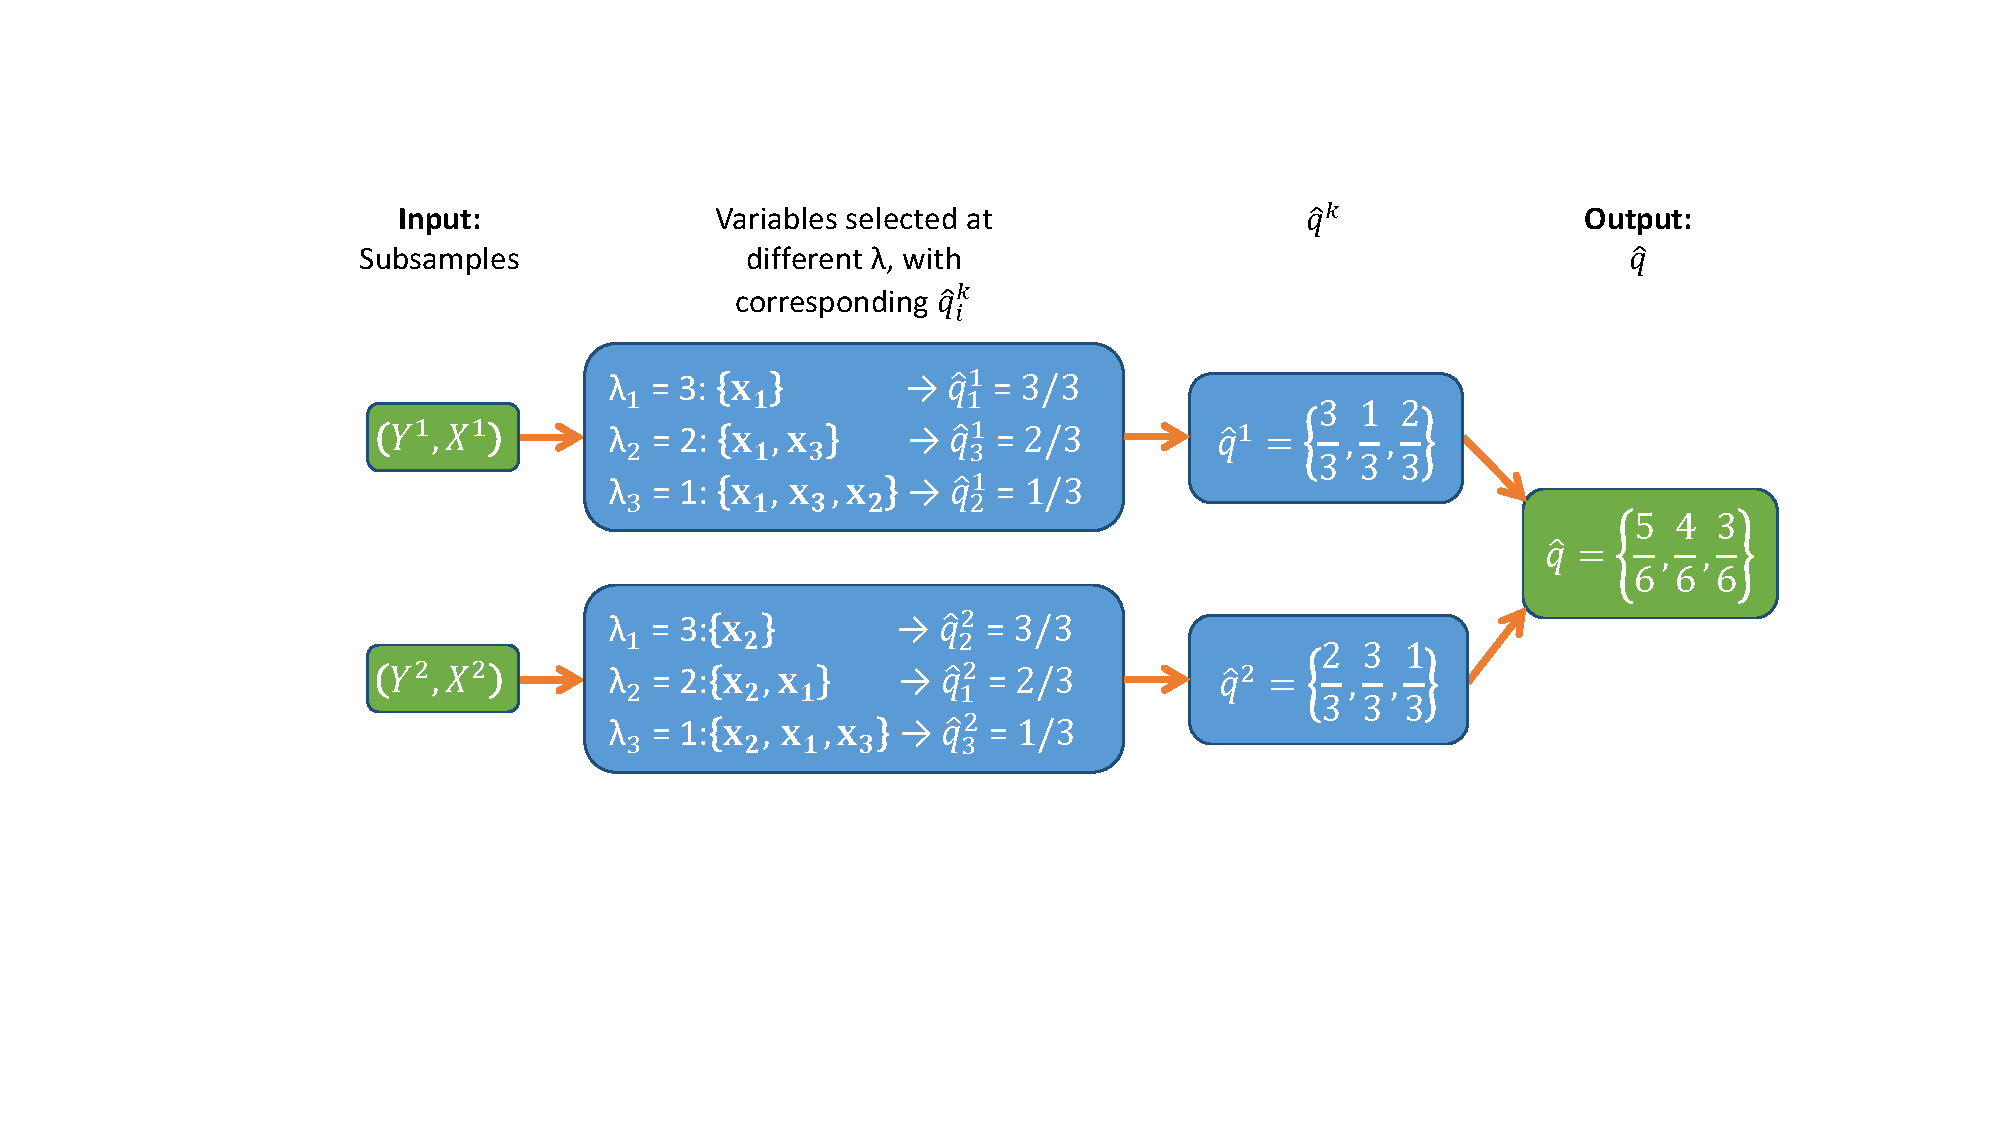
\includegraphics[width=0.66\paperwidth]{q_demo_3.pdf}
  %
  \caption{Computation of $\widehat{q}$ on 2 subsamples using coordinate descent.}
  %
  \label{fig:q_demo_3}
  %
\end{figure}

Algorithm~\ref{algo:APE-cd} estimates the average $L_0$ path via coordinate descent, serving the same purpose as Algorithm~\ref{algo:APE-lar}. Algorithm~\ref{algo:APE-cd} uses $\lambda$ to record the order that each variable enters the path. Consider the example in Figure~\ref{fig:q_demo_3}. To reparameterize the solution path, we denote $\lambda_s$ to be the $\lambda$ value that coordinate descent lasso includes $s$ variables, $\forall s\in \left( 0, \min \left\{ n/2, p \right\} \right]$, giving a sequence of $\lambda$ for grid search. In each subsample $\left( Y^k, X^k \right)$, we train a standard pathwise coordinate descent for lasso, allowing $\lambda$ to increase stepwise within the grid $\left\{\lambda_1, \ldots, \lambda_{ \min \left\{ n/2, p \right\} } \right\}$, where $\lambda_1 \geqslant \ldots \geqslant \lambda_{ \min \left\{ n/2, p \right\} }$. In Figure~\ref{fig:q_demo_3}, when $\lambda \leqslant \lambda_3$ at subsample $\left( Y^1, X^1 \right)$, all three variables are activated in the solution path, implying that $\widehat{q}^1_i \geqslant 1/3$ for all variables. When $\lambda$ increases to $\lambda_2$, only $\{\mathbf{x}_3, \mathbf{x}_1\}$ survive the harsher shrinkage, implying that they should be ranked higher than $\mathbf{x}_2$. As a result, $\widehat{q}^1_1, \widehat{q}^1_3 \geqslant 2/3$ and $\widehat{q}^1_2 = 1/3$. When $\lambda$ hits $\lambda_3$, only $\{\mathbf{x}_1\}$ remains activated, leaving $\widehat{q}^1_1 = 3/3$ and $\widehat{q}^1_3 = 2/3$. Subsequently, we apply the same method to each subsample, resulting in the same $\widehat{q}$ as Algorithm~\ref{algo:APE-lar}.

\section{Solar improvements over lasso variants, lasso rules, and variable screening \label{section:adv}}

\subsection{Comparison and generalization to lasso variants}

As shown above, solar averages and re-ranks lasso paths using the corresponding $L_0$ norm. Compared with lasso, solar has the following unique features.

\begin{itemize}

  \item Solar abandons shrinkage parameter optimization, determining a new $L_0$ path by discretizing the original lasso path. Compared with the $L_1$ path, the $L_0$ path is concentrated on dimensionality rather than parameter value and, hence, greatly boosts variable selection performance. More importantly, to avoid the NP-hard computation inherent in the traditional $L_0$ method (e.g., the best subset method via AIC/BIC), the $L_0$ path is computed from $L_1$-penalized optimization, improving speed even in large-scale and repetitive learning tasks (see Section~\ref{section:comp}).

  \item Because solar no longer needs to optimize $\lambda$ or $t$, it avoids the cross-validation conundrum. While unbiased and more generalizable than AIC/BIC, cross-validation faces a \emph{bias-variance trade-off} \citep{kearns1999algorithmic} and a \emph{stability issue} \citep{lim2016estimation}. Both issues significantly impact hyperparameter tuning and, hence, lasso selection performance (sparsity, stability, etc). Without a shrinkage parameter, solar relies on a jackknife- or bootstrap-like algorithm---training for $K$ rounds, removing $1/K$ of data each round---to stabilize the path.

\end{itemize}

Because it is trained by least-angle regression or coordinate descent, solar can easily be generalized to many lasso-type problems. For example,

\begin{itemize}
  %
  \item `Grouped solar' is invoked by requiring some variables to be simultaneously selected into the solution path;
  %
  \item `Adaptive solar' is obtained by weighting variable rankings in the average $L_0$ path according to their OLS coefficients;
  %
  \item `Solar elastic net' or `fused solar' is derived by replacing the coordinate descent loss function in Algorithm~\ref{algo:APE-cd} with the $L_1$-$L_2$ loss
    %
    \begin{equation}
      %
      \left\Vert Y -X\beta \right\Vert_2^2 + \lambda^{(1)} \left\Vert \beta \right\Vert_1 + \lambda^{(2)} \left\Vert \beta \right\Vert_2^2
      %
    \end{equation}
    %
    or fused loss
    %
    \begin{equation}
      %
      \left\Vert Y -X\beta \right\Vert_2^2 + \lambda^{(1)} \left\Vert \beta \right\Vert_1 + \lambda^{(2)} \sum_{j=2}^{p} \left\vert \beta_j - \beta_{j-1} \right\vert_1.
      %
    \end{equation}
    %
\end{itemize}

Most importantly, because they use the same optimization methods, many lasso enhancements (e.g., lasso rules, post-lasso hypothesis testing) can be applied to solar. Rather than competing with the lasso enhancements, solar supplements them, further improving variable selection efficiency and performance in large-scale applications.

\subsection{Solar advantages on post-selection hypothesis testing}

As we show in Section~\ref{section:comp}, solar is superior to lasso-type algorithms in terms of selection sparsity, accuracy, and efficiency. In addition, solar is amenable to post-selection testing. Because the lasso tests \citep{lockhartall14, taylor2014exact} are based on least-angle regression, they may be adapted to solar. More interestingly, it is straightforward to adapt the data-splitting tests \citep{wasserman2009high,meinshausen2009p} to solar \hl{for a further performance boost}. We illustrate this point using Example~1.

\smallskip
\noindent
\textbf{Example 1.} Suppose the DGP is
%
\begin{equation}
  Y = 2 \mathbf{x}_0 + 3 \mathbf{x}_1 + 4 \mathbf{x}_2 + 5 \mathbf{x}_3 + 6 \mathbf{x}_4 + \sum_{j=5}^{p} 0 \cdot \mathbf{x}_j + e,
\end{equation}
%
\hl{where $\mathbf{x}_i$, $i=0,\dots,p$,} are standard Gaussian with pairwise correlations of $0.5$ and $e$ is a standard Gaussian noise. Post-selection tests are typically applied with sufficiently large $n$, so $p/n=50/100$. In this setting, forward regression (FR) selects $\left[\mathbf{x}_4, \mathbf{x}_3, \mathbf{x}_2, \mathbf{x}_1, \mathbf{x}_0, \mathbf{x}_{45}, \mathbf{x}_{8}, \mathbf{x}_{40}, \mathbf{x}_{6}, \mathbf{x}_{39}, \mathbf{x}_{11}, \mathbf{x}_{34}, \mathbf{x}_{5} \right]$ using BIC score minimization. By contrast, solar selects only $\left[\mathbf{x}_4, \mathbf{x}_3, \mathbf{x}_2, \mathbf{x}_1, \mathbf{x}_0, \mathbf{x}_{45}, \mathbf{x}_{40} \right]$. We then conduct post-FR and post-solar t-tests and compare the results to the OLS regression of $Y$ on the $\mathbf{x}_i$.

After standardizing the $\mathbf{x}_i$ and $\mathbf{Y}$, the sample regression coefficient is identical to the corresponding conditional correlation. Both the t-test results and FR selection decisions are largely based on the sample regression coefficient absolute values; keeping variables with large values and purging the rest. Hence, the variables selected by FR also have low p-values on the current sample, implying that direct, post-FR t-tests overfit the sampling randomness that also affects the variable selection algorithm (referred to as `p-value overfitting'). The main problem here is that there is no sample change between the FR sample and the post-FR test sample.

To solve this issue, we improve the data-splitting tests by merging the \citet{bousquet2002stability} method---a jackknife-type algorithm---and the \citet{diciccio2020exact} theoretical results, as follows: after solar selection on the whole sample, we randomly divide the sample into $K$ folds, remove each fold in turn, and compute the t- and p-values of post-solar OLS on the remaining $K-1$ folds. We calculate the average t-, p-values, and standard errors in $K$ rounds resulting in the \emph{$K$-fold average}. In this example we focus on $K=2$, which we refer to as the \emph{hold-out average}. Our approach has the following advantages over the \citet{wasserman2009high} and \citet{meinshausen2009p} methods:

\begin{itemize}
  %
  \item The \citet{meinshausen2009p} method requires a computationally costly, bootstrap-like repetition: each bootstrap subsample is split, one portion is used for selection, the  other for testing. By contrast, the hold-out average only uses one realization of variable selection and two post-selection tests. This is useful when the dimensionality or data size is very large (see the simulation runtime comparison at section~\ref{section:comp}).
  %
  \item Rather than using a portion of the data, the hold-out average uses the whole sample for variable selection, improving variable selection accuracy.
  %
  \item The hold-out average only relies on the concentration inequalities for averaging testing performance. Hence, the hold-out average is consistent with the \citet{diciccio2020exact} framework and inherits a number of elegant theoretical properties. Most importantly, the hold-out averaging test with $K=2$ splits the data into two disjoint portions, which removes the autocorrelation of t- and p-values across rounds and further simplifies the \citet{diciccio2020exact} theoretical derivation.\footnote{Due to the similarity between $K$-fold CV and $K$-fold averaging, $K \leqslant 10$ \citep{friedman2001elements} is also recommended for controlling the autocorrelation among t- or p-values across different rounds.}
  %
\end{itemize}

As shown in Table~\ref{table:post-selection-test}, the hold-out average t-values for $\left[\mathbf{x}_4, \mathbf{x}_3, \mathbf{x}_2, \mathbf{x}_1, \mathbf{x}_0\right]$ are very similar to their OLS counterparts while the hold-out average t-values for $\left[\mathbf{x}_{40}, \mathbf{x}_{45} \right]$ are lower, which leads to purging $\mathbf{x}_{40}$ and $\mathbf{x}_{45}$. We repeat the simulation 200 times and the results, summarized in Figure~\ref{fig:t_value_compare}, confirm that improvements in the hold-out average are not simply due to chance. It is important to note that OLS uses all of the sample and has $50$ residual degrees of freedom whereas the hold-out average uses only 50\% of the sample in each round and consequently has $30$-$40$ degrees of freedom. Thus, the hold-out average naturally produces slightly lower t-values for $\left[\mathbf{x}_4, \mathbf{x}_3, \mathbf{x}_2, \mathbf{x}_1, \mathbf{x}_0\right]$ and the t-value boxplots for the hold-out average are slightly less concentrated than the OLS boxplots. Simulations in Section~\ref{subsection:suml1}, show that solar supplemented with the hold-out average purges almost all of the redundant variables while retaining all of the informative variables. $\blacksquare$

%\smallskip
\begin{table}[h]
\centering
\caption{Comparison of post-selection t tests between FR, hold-out average, and OLS.}
\label{table:post-selection-test}
\renewcommand{\arraystretch}{0.7}
  \begin{tabular}{l............}
    \toprule
    & \multicolumn{3}{c}{post-FR} & \multicolumn{3}{c}{hold-out average} & \multicolumn{3}{c}{classical OLS} \\
    \cmidrule(lr){2-4} \cmidrule(lr){5-7} \cmidrule(lr){8-10}
    & \multicolumn{1}{c}{$se$} & \multicolumn{1}{c}{$t$} & \multicolumn{1}{c}{$P>\left\vert t \right\vert$ } & \multicolumn{1}{c}{$se$} & \multicolumn{1}{c}{$t$} & \multicolumn{1}{c}{$P>\left\vert t \right\vert$} & \multicolumn{1}{c}{$se$} & \multicolumn{1}{c}{$t$} & \multicolumn{1}{c}{$P>\left\vert t \right\vert$} \\
    \cmidrule{1-10}
    $\mathbf{x}_0$ & 0.12 & 15.68 & 0 & 0.18 & 11.34 & 0 & 0.19 & 9.85 & 0 \\
    $\mathbf{x}_1$ & 0.14 & 20.06 & 0 & 0.22 & 12.76 & 0 & 0.23 & 12.05 & 0 \\
    $\mathbf{x}_2$ & 0.14 & 28.11 & 0 & 0.21 & 18.22 & 0 & 0.20 & 19.45 & 0 \\
    $\mathbf{x}_3$ & 0.13 & 39.19 & 0 & 0.20 & 24.48 & 0 & 0.20 & 25.08 & 0 \\
    $\mathbf{x}_4$ & 0.13 & 42.34 & 0 & 0.21 & 27.36 & 0 & 0.20 & 28.15 & 0 \\
    $\mathbf{x}_{40}$ & 0.12 & 2.59 & 0.01 & 0.19 & 1.90 & 0.18 & 0.18 & 2.36 & 0.02 \\
    $\mathbf{x}_{45}$ & 0.13 & 2.30 & 0.02 & 0.21 & 1.19 & 0.25 & 0.19 & 1.60 & 0.12 \\
    \bottomrule
  \end{tabular}
\end{table}
\smallskip


\begin{figure}[h]
%
  \centering
%
  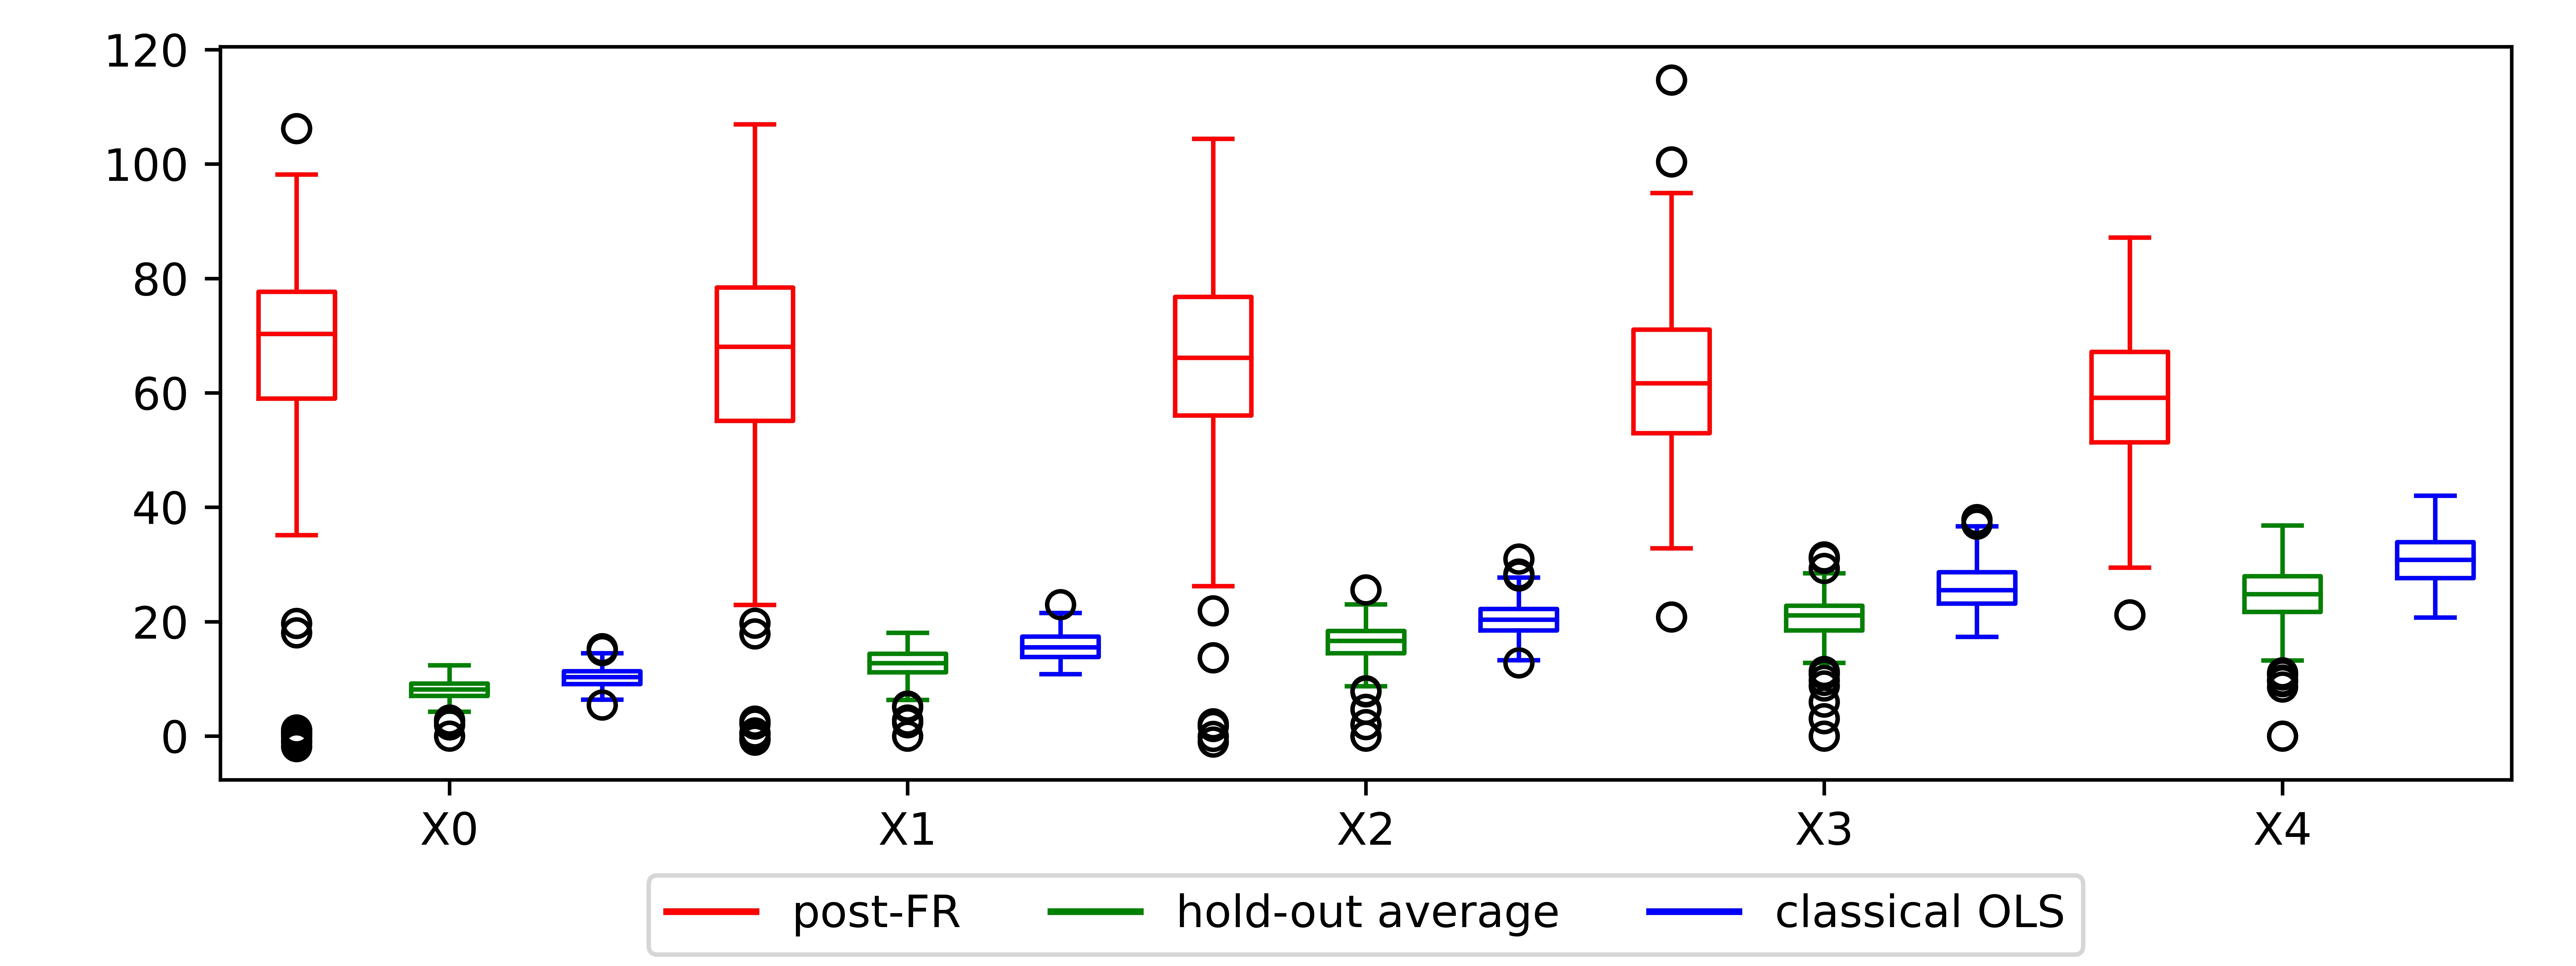
\includegraphics[width=0.7\paperwidth]{t_value_compare.jpg}
%
  \caption{Boxplots of post-selection t values from FR, hold-out average, and OLS.}
%
  \label{fig:t_value_compare}
%
\end{figure}

While the hold-out average procedure can be applied to other methods, solar has several intrinsic advantages.

\begin{itemize}
  %
  \item Firstly, to ensure accurate tests with only half the sample, it is important to retain residual degrees of freedom, implying that variable selection must be as sparse and accurate as possible. As shown in Sections~\ref{section:comp} and \ref{section:application}, sparse and accurate selection is one of the benefits of solar.
  %
  \item Secondly, the residual degrees of freedom are less than $p$ in high-dimensional data. Hence, when applying post-selection tests to address the selection of redundant variable or the omission of informative variables, we must decide which $\beta_i$ to test. \citet[Theorem~2]{zhang09} suggests that the earlier a variable enters the path, the more likely it is to be informative, implying we should test variables that rank higher in priority. \hl{Compared to FR and lasso paths, the solar ranking from the average $L_0$ path is robust to settings of the irrepresentable condition, sampling noise, multicollinearity, and other issues. Hence, solar also provides guidance on $\beta_i$ testing priority.}
  %
\end{itemize}

To conclude, Example~1 illustrates that the hold-out average may significantly reduce the severity of `p-value overfitting' while utilizing as many data points as possible for selection and testing. This method helps reduce the severity of informative variable omission or redundant variable inclusion.

\subsection{Solar advantages under complicated dependence structures\label{section:example}}

Indeed, solar has another advantage: the average $L_0$ solution path offers additional robustness against outliers, multicollinearity, and noise in high-dimensional spaces. Thus, solar is likely to be more reliable than other variable selection methods under complicated dependence structures. We illustrate the point with the following two Bayesian network examples.

\begin{figure}[h]
%
  \centering
  %
  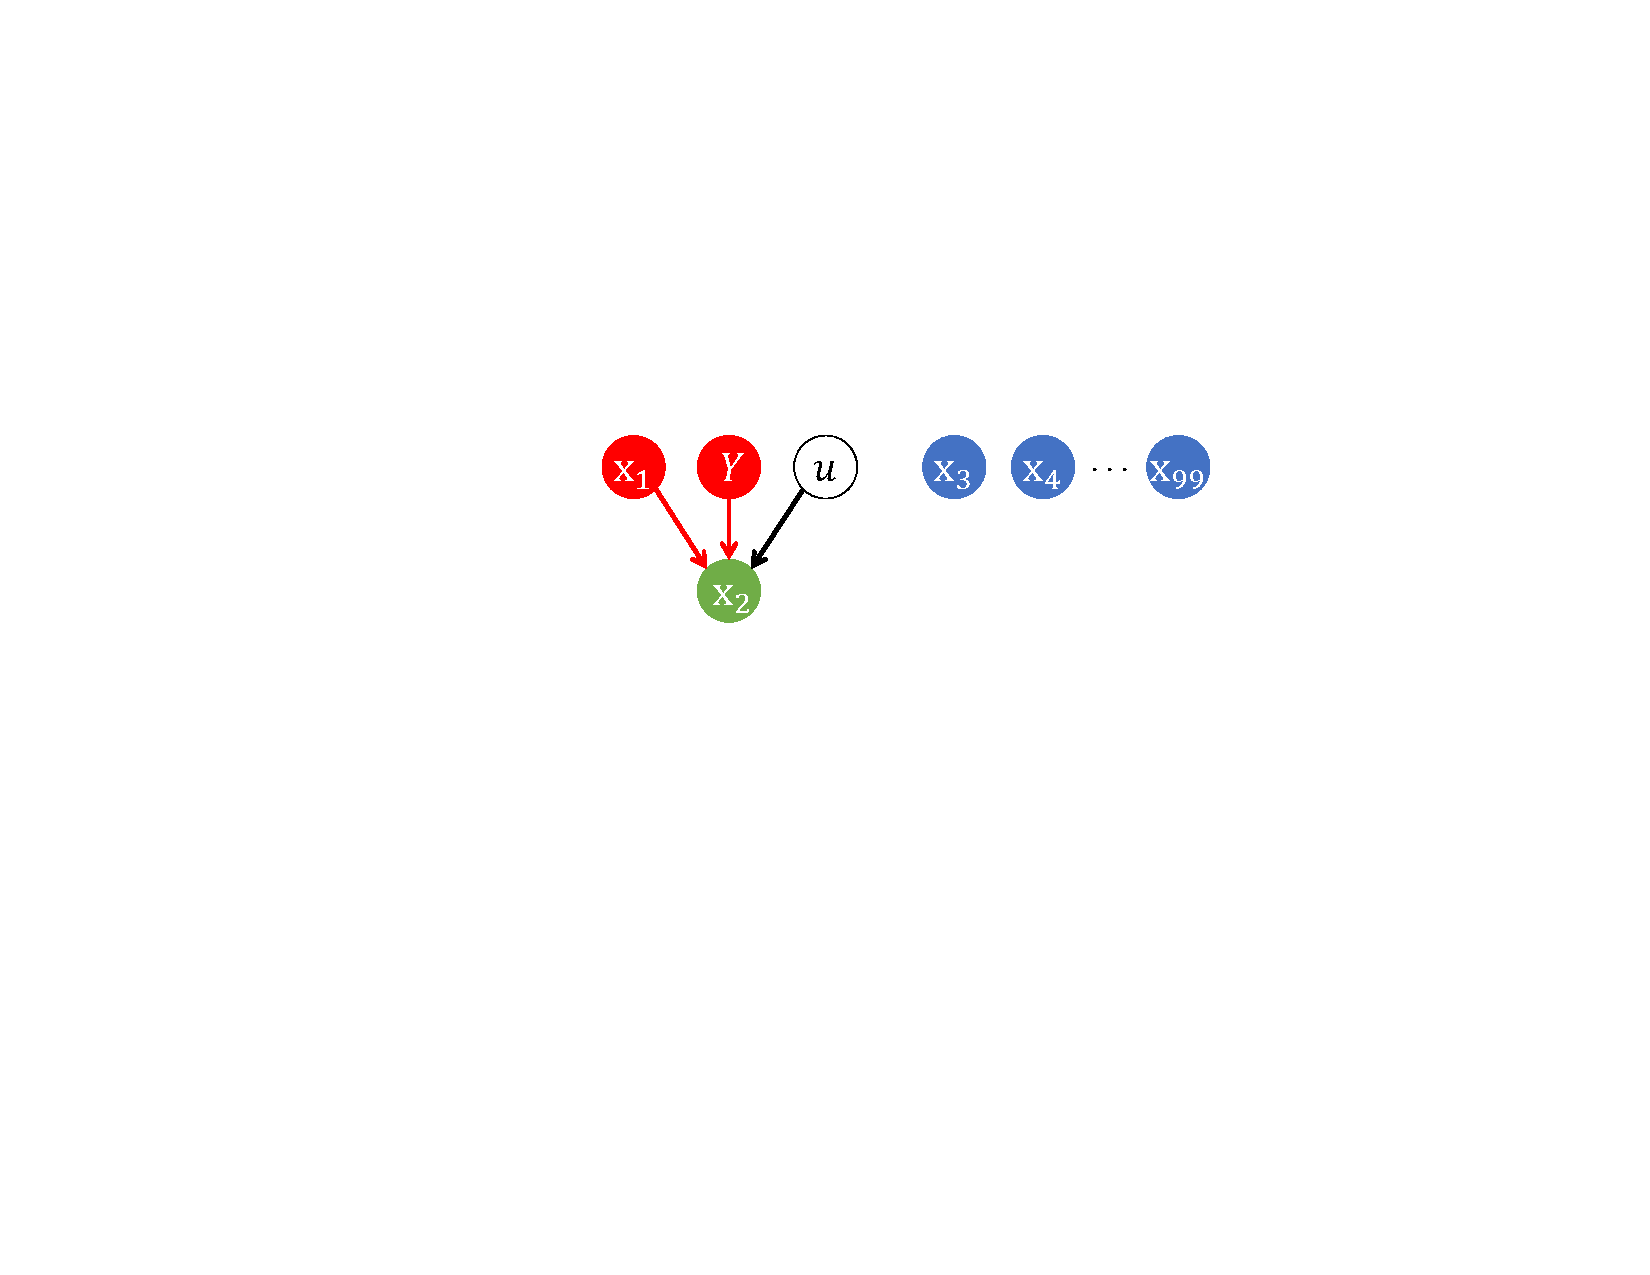
\includegraphics[width=0.35\paperwidth]{uncond_example.pdf}
  %
  \caption{Y is unconditionally uncorrelated to an informative $\mathbf{x}_1$.}
  %
  \label{fig:uncond_example}
%
\end{figure}

Consider the non-standard regression case in Figure~\ref{fig:uncond_example}, which depicts a common empirical regression problem: \emph{informative variables} that are \emph{unconditionally uncorrelated to} $Y$ in the DGP. \hl{For example, in biostatistics, concussion ($\mathbf{x}_1$) or a brain tumor ($Y$) may cause headaches ($\mathbf{x}_2$), implying that concussion history is important in brain tumor diagnosis. Hence, $\mathbf{x}_1$ and $\mathbf{x}_2$ are informative variables for $Y$, even though $\mathbf{x}_1$ and $Y$ are independent. Example~4} shows that solar is more reliable than post-lasso rules and variable screening.

\smallskip
\noindent
\textbf{Example 2.} In Figure~\ref{fig:uncond_example}, there are $100$ variables and $\mathbf{x}_2$ is (causally) generated by its parents $\left\{ \mathbf{x}_1, Y \right\}$ as follows,
%
\begin{equation}
  %
  \mathbf{x}_2 = \alpha_1 \mathbf{x}_1 + \alpha_2 Y + u,
  %
  \label{eqn:collider_1}
  %
\end{equation}
%
where $\mathbf{x}_1$ is unconditionally uncorrelated with $Y$, $\mathbf{x}_1$ and $Y$ are both unconditionally and conditionally uncorrelated with the redundant variables, $\left\{\alpha_1, \alpha_2 \right\}$ are population regression coefficients, and $u$ is a Gaussian noise term. If $Y$ is chosen to be the response variable, we have the population regression equation
%
\begin{equation}
  %
  Y = -\frac{\alpha_1}{\alpha_2} \mathbf{x}_1 + \frac{1}{\alpha_2} \mathbf{x}_2 - \frac{1}{\alpha_2}u.
  %
  \label{eqn:collider_2}
  %
\end{equation}
%
Note that $\mathbf{x}_1$ and $\mathbf{x}_2$ are both informative variables for $Y$. However, since $\mathbf{x}_1$ is unconditionally uncorrelated with $Y$ in the population, some post-lasso rules [such as the strong rule \citep{tibshirani2012strong} and the safe rule \citep{ghaoui2010safe}] may be prone to purging $\mathbf{x}_1$ incorrectly. Given the value of shrinkage parameter $\lambda$ in a grid search, the base strong rule and the safe rule for lasso to purge any selected variable, respectively, satisfies (\ref{eqn:safe_rule}) and (\ref{eqn:strong_rule}):
%
\begin{eqnarray}
  %
  \left\vert \mathbf{x}_i^T Y \right\vert < & \lambda - \left\Vert \mathbf{x}_i \right\Vert_2 \left\Vert Y \right\Vert_2 \frac{\lambda_{max} - \lambda} {\lambda_{max}} ; \label{eqn:safe_rule} \\
  %
  \left\vert \mathbf{x}_i^T Y \right\vert < & 2\lambda - \lambda_{max} , \label{eqn:strong_rule}
  %
  \label{eqn:post_estmation_rule}
  %
\end{eqnarray}
%
where the $\mathbf{x}_i$ are standardized and $\lambda_{max}$ is the value of $\lambda$ that purges all the variables. Both rules are based on the unconditional covariance between $\mathbf{x}_i$ and $Y$. For a given value of $\lambda$ (typically selected by CV), lasso likely will select $\mathbf{x}_1$ and $\mathbf{x}_2$ along with some redundant variables from $\left\{ \mathbf{x}_3, \ldots, \mathbf{x}_{99} \right\}$ (since the DGP does not violate any IRC). Since $\mathrm{corr} \left( \mathbf{x}_1, Y \right) = \mathrm{corr} \left( \mathbf{x}_3, Y \right) =  \cdots = \mathrm{corr} \left( \mathbf{x}_{99}, Y \right) = 0$ in the population, the sample value of $\left\vert \mathbf{x}_1^T Y \right\vert$ will be approximately as small as the $\left\vert \mathbf{x}_i^T Y \right\vert$ of any redundant variable. Put another way, $\mathbf{x}_1$ cannot be distinguished from the redundant variables by the value of $\left\vert \mathbf{x}_i^T Y \right\vert$. To ensure $\mathbf{x}_1$ is not purged by (\ref{eqn:safe_rule}) or (\ref{eqn:strong_rule}), both $\lambda - \left\Vert \mathbf{x}_1 \right\Vert_2 \left\Vert Y \right\Vert_2 \frac{\lambda_{max} - \lambda} {\lambda_{max}}$ and $2\lambda - \lambda_{max}$ must be smaller than $\left\vert \mathbf{x}_1^T Y \right\vert$. However, this will lead to two problems. First, decreasing the right-hand side of (\ref{eqn:safe_rule}) and (\ref{eqn:strong_rule}) will reduce the value of $\lambda$, implying that lasso will select more redundant variables. Second, since $\left\vert \mathbf{x}_1^T Y \right\vert$ will be approximately as small as the $\left\vert \mathbf{x}_i^T Y \right\vert$ of any redundant variable selected by lasso, not purging $\mathbf{x}_1$ (by reducing both right-hand side terms) may result in (\ref{eqn:safe_rule}) and (\ref{eqn:strong_rule}) retaining redundant variables.

Variable screening methods \citep{fan2008sure} may also be prone to selecting redundant variables. Screening ranks variables decreasingly based on the absolute values of their unconditional correlations to $Y$, selecting the top $w$ variables (with $w$ selected by CV, bootstrap or BIC). Since $\mathrm{corr} \left( \mathbf{x}_2, Y \right) \neq 0$ in the population, screening will rank $\mathbf{x}_2$ highly. However, it may not rank $\mathbf{x}_1$ highly because $\mathrm{corr} \left( \mathbf{x}_1, Y \right) = 0$ in the population. Thus, some redundant variables may be ranked between $\mathbf{x}_2$ and $\mathbf{x}_1$, implying that if both $\mathbf{x}_1$ and $\mathbf{x}_2$ are selected, screening will select redundant variables.

The average $L_0$ solution path will not suffer the same problem. For convenience, assume $-\alpha_1 / \alpha_2 > 0$ and $p/n = 100/200$ or smaller. For lars, as we increase $\left\Vert \beta_2 \right\Vert_1$ at stage~1 (i.e., as we `partial' $\mathbf{x}_2$ out of $Y$), the unconditional correlation between $Y - \beta_2 \mathbf{x}_2$ and $\mathbf{x}_1$ will increase above $0$ significantly while the marginal correlation between $Y - \beta_2 \mathbf{x}_2$ and any redundant variable will remain approximately $0$. Thus, in the $L_0$ solution path and, hence, the average $L_0$ solution path, $\mathbf{x}_1$ will be included immediately after $\mathbf{x}_2$ is included. $\blacksquare$

\citet{fan2008sure} and \citet{barut2016conditional} propose three solutions for the Example~2 variable screening issue. However,

\begin{itemize}
  %
  \item the first approach \citep[Section~2.2 and~3]{barut2016conditional} assumes the identity of $\mathbf{x}_2$ in Example~2 and Figure~\ref{fig:uncond_example} is known (also called a \emph{collider} in Bayesian network or probabilistic graph modelling, \citet{barut2016conditional} call it a \emph{hidden signature} variable and denote it by $X_c$), which is unlikely to be realistic in practical applications;
  %
  \item the second approach \citep[Section~1 and~2.2]{barut2016conditional} suggests that randomly trying out several variables as colliders may be beneficial. The logic is straightforward: randomly trying out the wrong variable to be a collider ($\mathbf{x}_2$ in Example~2 and Figure~\ref{fig:uncond_example}) is harmless because conditioning on that variable will not make $corr(Y,\mathbf{x}_1) \neq 0$, nor will it cause the selection of a redundant variable. Moreover, by repeatedly randomly trying out variables, there is a non-zero probability the correct collider is eventually uncovered, producing a statistically significant $corr(Y,\mathbf{x}_1) \neq 0$. However, using multiple trials may be inefficient and computationally expensive, especially with high-dimensional data. \hl{Even though $corr(Y, \mathbf{x}_1) \neq 0$ after simultaneously trying out multiple variables (say $\left\{\mathbf{x}_2, \mathbf{x}_3, \ldots, \mathbf{x}_{99} \right\}$), we still must determine whether any of $\left\{\mathbf{x}_2, \mathbf{x}_3, \ldots, \mathbf{x}_{99} \right\}$ are redundant, leaving variable selection at a possible loose end.}
  %
\end{itemize}

\medskip

The next example illustrates another common problem in empirical regression: \emph{redundant variables} that are \emph{unconditionally correlated to} $Y$ in the DGP. In Figure~\ref{fig:cond_example}, \hl{the problem occurs because $\mathbf{x}_3$ and $Y$ are determined by common variables. For example, house rent ($Y$) and food expenditure ($\mathbf{x}_3$) are both determined by income ($\mathbf{x}_1$) and saving ($\mathbf{x}_2$), yet $\mathbf{x}_3$ is redundant if $\mathbf{x}_1$ and $\mathbf{x}_2$ have already been used to predict $Y$. In the next example, we demonstrate that} the strong rule, base rule, and variable screening methods may have difficulty purging the redundant $\mathbf{x}_3$ even when IRC is satisfied. By contrast, solar is more reliable.

\begin{figure}[h]
  %
    \centering
    %
    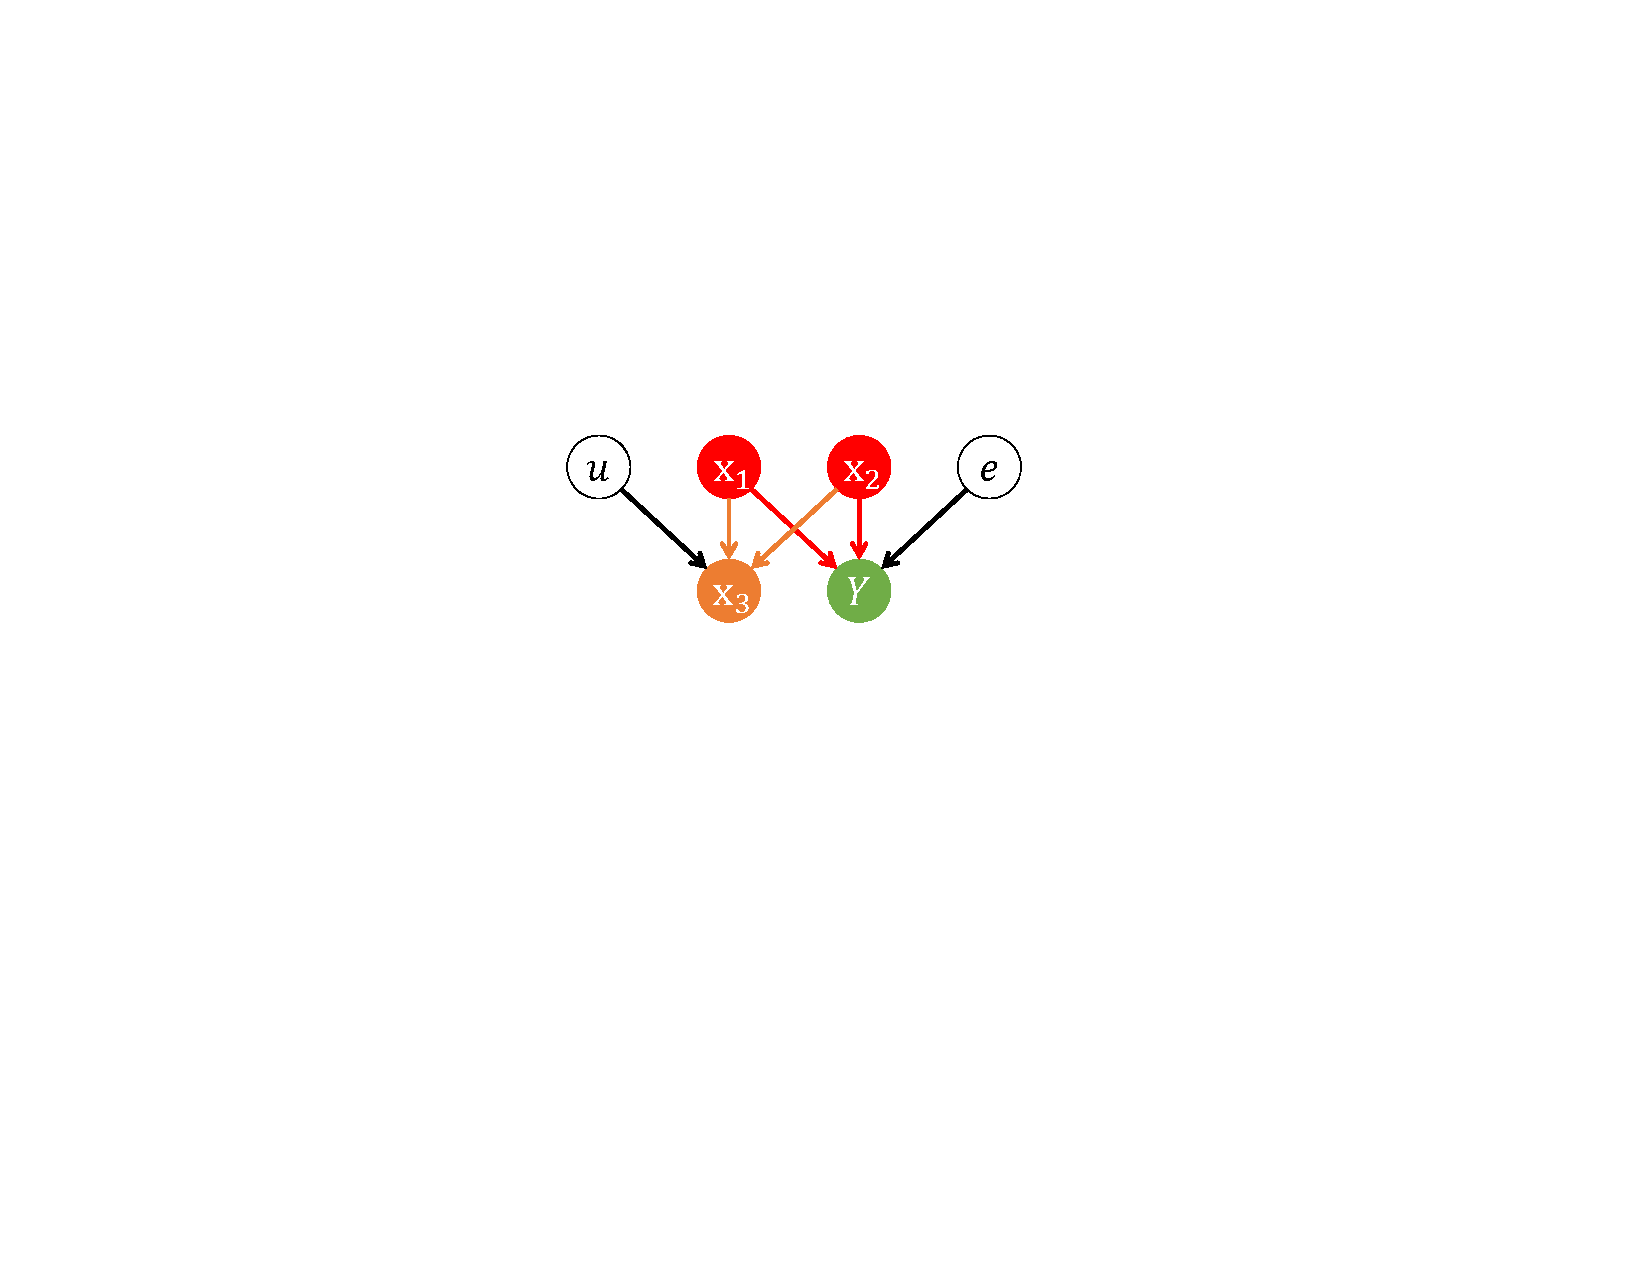
\includegraphics[width=0.35\paperwidth]{example3.pdf}
    %
    \caption{$Y$ is unconditionally correlated with redundant $\mathbf{x}_3$.}
    %
    \label{fig:cond_example}
  %
  \end{figure}

\smallskip
\noindent
\textbf{Example 3.} Consider the following confounding structure,
%
\begin{equation}
	%
	\begin{cases}
	%
    \mathbf{x}_3 = \frac{1}{3} \mathbf{x}_1 + \frac{1}{3} \mathbf{x}_2 + \frac{\sqrt{7}}{3} u, \\
    %
    Y = \frac{7}{10} \mathbf{x}_1 +  \frac{2}{10} \mathbf{x}_2 +  \frac{\sqrt{47}}{10} e. \\
    %
	\end{cases}
	%
	\label{eqn:example_4}
	%
\end{equation}
%
As shown in Figure~\ref{fig:cond_example}, $\mathbf{x}_1$ and $\mathbf{x}_2$ cause both $Y$ and $\mathbf{x}_3$, implying that $\mathbf{x}_3$ is unconditionally correlated to $Y$; $\mathbf{x}_1$, $\mathbf{x}_2$, $u$ and $e$ are independent; $\mathbf{x}_3$ is independent from $e$; $Y$ is independent from $u$; and all variables are standardized. When $n$ is large and the sample correlations close to their population values, the sample marginal correlations to $Y$ can be ranked in decreasing order,
%
\begin{equation}
  %
  \begin{aligned}
    %
    \mathrm{corr} \left( \mathbf{x}_1, Y \right)  = & \;0.7 \\
    %
    \mathrm{corr} \left( \mathbf{x}_3, Y \right)  = & \;\mathrm{corr} \left( \frac{1}{3} \mathbf{x}_1 + \frac{1}{3} \mathbf{x}_2, \frac{7}{10} \mathbf{x}_1 +  \frac{2}{10} \mathbf{x}_2 \right)
    %
    = 0.3. \\
    %
    \mathrm{corr} \left( \mathbf{x}_2, Y \right)  = & \;0.2 \\
    %
  \end{aligned}
  %
\end{equation}
%
Because $\mathbf{x}_2$ ranks below $\mathbf{x}_1$ and $\mathbf{x}_3$ in terms of marginal correlations to $Y$, the variable screening method will have to select all $3$ variables, including the redundant $\mathbf{x}_3$, to avoid omitting $\mathbf{x}_2$. Similarly, the base strong rule and safe rule may also have difficulty purging $\mathbf{x}_3$. Because $\mathrm{corr} \left( \mathbf{x}_3, Y \right)$ is larger than $\mathrm{corr} \left( \mathbf{x}_2, Y \right)$, if lasso selects both $\mathbf{x}_3$ and $\mathbf{x}_2$ and we use the base strong rule or the safe rule to purge $\mathbf{x}_3$, we will also have to purge $\mathbf{x}_2$.

Forward regression, solar and lasso will not make the same errors. Because (\ref{eqn:example_4}) does not violate the IRC, variable-selection consistency of forward regression, lasso and lars is assured by the theoretical results of \citet{zhang09} and \citet{zhaoyu06}. Specifically in forward regression, $\mathbf{x}_1$ will be included  at the first stage. After controlling for $\mathbf{x}_1$, the partial correlations to $Y$ of both $\mathbf{x}_2$ and $\mathbf{x}_3$ can be ranked in decreasing order as follows (when $n$ is large),
%
\begin{equation}
  %
  \begin{aligned}
    %
    \mathrm{corr} \left( \mathbf{x}_2, Y \vert \mathbf{x}_1 \right)  = & \;\mathrm{corr} \left( \mathbf{x}_2, \frac{2}{10} \mathbf{x}_2 \right)
    %
    = 0.2. \\
    %
    \mathrm{corr} \left( \mathbf{x}_3, Y \vert \mathbf{x}_1 \right)  = & \;\mathrm{corr} \left( \frac{1}{3} \mathbf{x}_1 + \frac{1}{3} \mathbf{x}_2, \frac{2}{10} \mathbf{x}_2 \right)
    %
    = 0.0667. \\
    %
  \end{aligned}
  %
\end{equation}
%
Thus, at the second stage, forward regression will include $\mathbf{x}_2$, not $\mathbf{x}_3$. After controlling for both $\mathbf{x}_1$ and $\mathbf{x}_2$, the remaining variation in $Y$ comes from $e$, which $\mathbf{x}_3$ cannot explain. As a result, CV or BIC will terminate forward regression after the second stage and $\mathbf{x}_3$ will not be selected. Similarly, because solar relies on the average $L_0$ path, it will include $\mathbf{x}_1$ and $\mathbf{x}_2$ but not $\mathbf{x}_3$. $\blacksquare$

\smallskip
Essentially, the strong rule, safe rule, and variable screening struggle in these two examples because they rely on unconditional correlations to $Y$, whereas informative variables in regression analysis are defined in terms of conditional correlations. In many scenarios, unconditional and conditional correlations are aligned. However, when they are not, variable selection based conditional correlation is better placed to select the informative variables.

\citet{fan2008sure} propose the following solutions. That approach requires repeating the following steps: running variable screening on $Y$, selecting variables having high unconditional correlations with $Y$, and running a lasso of the residuals on the dropped variables. In contrast, by using conditional correlation ranking, solar completes variable selection in a single realization, reducing the computational cost in large-scale applications. Moreover, the \citet{fan2008sure} approach does not solve the Example~3 problem. In their first step, variables with high unconditional correlations to $Y$ (including the redundant $\mathbf{x}_3$) will be selected, implying the inclusion of invalid variables. The issue will be exacerbated if $Y$ has multiple $\mathbf{x}_3$-like siblings within a complicated dependence structure: the multicollinearity will produce inaccurate estimations of the regression coefficients and standard errors in finite samples. In short, solar is likely to be more computationally efficient and better at variable selection under complicated dependence structures.

%%%%%%%%%%%%%%%%%%%%%%%%%%%%%%%%%%%%%%%%%%
%%%%%%%%%%%%%%%%%%%%%%%%%%%%%%%%%%%%%%%%%%
%%%%% irrepresentable cond of solar %%%%%%
%%%%%%%%%%%%%%%%%%%%%%%%%%%%%%%%%%%%%%%%%%
%%%%%%%%%%%%%%%%%%%%%%%%%%%%%%%%%%%%%%%%%%

\subsection{Solar robustness to different settings of the IRC \label{subsection:irc}}

Here we illustrate that, compared to lasso, solar has superior robustness to different settings of the \emph{irrepresentable condition (IRC)}, which is considered to be sufficient and almost neccessary for accurate lasso variable selection \citep{zhang09}. We skip lasso rules and variable screening here since, as discussed above, their selection accuracy may be affected by their reliance on unconditional correlation to $Y$. Following \citet{zhang09}, we define IRC as follows,

\begin{definition}[IRC]
  Given $F \subset \left\{ 1, \ldots, p \right\}$, define $X_F$ to be the $n \times \left\vert F \right \vert$ matrix with only the full set of informative variables. Define
  %
    \begin{align}
    %
    \mu \left( F \right) = & \max \left\{ \left\Vert \left( \left( X_F \right)^T X_F \right)^{-1} \left( X_F \right)^T \mathbf{x}_j \right\Vert_1 \; \vert \; \forall j \not\in F \right\}. \notag
    %
    \end{align}
  %
  Given a constant $1 \geqslant \eta > 0$, the \emph{strong} irrepresentable condition is satisfied if $\mu \left( F \right) \leqslant 1 - \eta$ and the \emph{weak} irrepresentable condition is satisfied if $\mu \left( F \right) < 1$.$\blacksquare$
\end{definition}

\smallskip
We follow the simulation of \citet{zhaoyu06} and slightly modify the Example~3 DGP. Here, $n = 200$, $p = 50$, and $[\mathbf{x}_0, \ldots, \mathbf{x}_4, \mathbf{x}_6, \ldots, \mathbf{x}_{50}]$ is generated from a zero-mean, unit-variance multivariate Gaussian distribution, where all the correlation coefficients are $0.5$. The DGP of $Y$ and $\mathbf{x}_5$ is
\begin{equation}
	%
	\begin{cases}
	%
    \mathbf{x}_5 = \omega \mathbf{x}_0 + \omega \mathbf{x}_1 + \gamma\cdot \sqrt{1 - 2\omega^2} \\
    %
    Y = 2 \mathbf{x}_0 + 3\mathbf{x}_1 + 4 \mathbf{x}_2 + 5 \mathbf{x}_3 + 6 \mathbf{x}_4 + e \\
    %
	\end{cases}
	%
	\label{eqn:dgp_x5}
	%
\end{equation}
%
where $\omega \in \mathbb{R}$, while $\gamma$ and $e$ are both standard Gaussian noise terms, independent from each other and all the other variables. Compared with Example~3, this DGP has more redundant signals, increasing the challenge of purging redundant variables. The example also makes it straightforward to control the value of $\mu \left( F \right)$ with $\omega$.

\begin{figure}
  %
  \centering
  %
  \subfloat[\label{fig:solar_ic_type-II1}$\omega = 1/4,\;\mu\left(F\right)=1/2$, lasso]
  {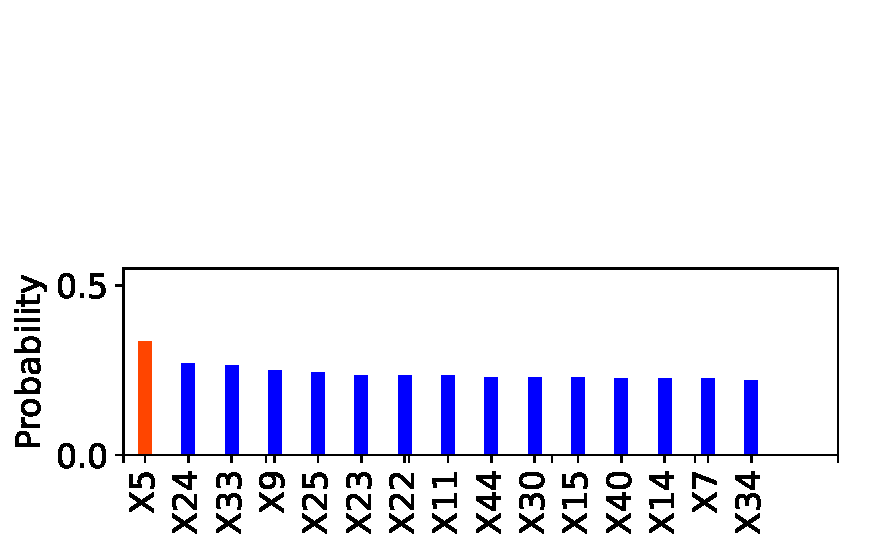
\includegraphics[width=0.25\paperwidth]{acc_plot_top20_ic_25_False_lars-crop.pdf}}
  %
  \subfloat[\label{fig:solar_ic_type-II2}$\omega = 1/3,\;\mu\left(F\right)=2/3$, lasso]
  {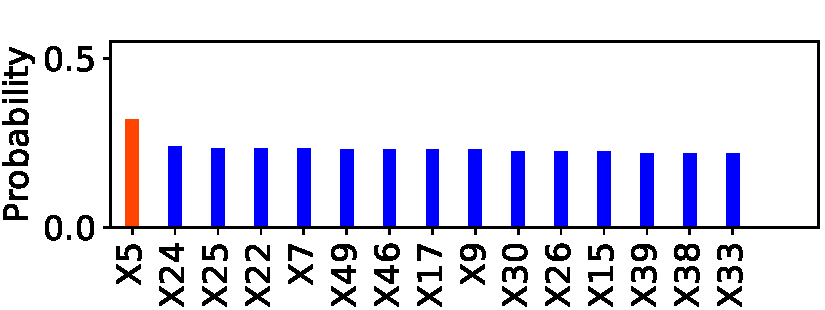
\includegraphics[width=0.25\paperwidth]{acc_plot_top20_ic_33_False_lars-crop.pdf}}
  %
  \subfloat[\label{fig:solar_ic_type-II3}$\omega = 1/2,\;\mu\left(F\right)=1$, lasso]
  {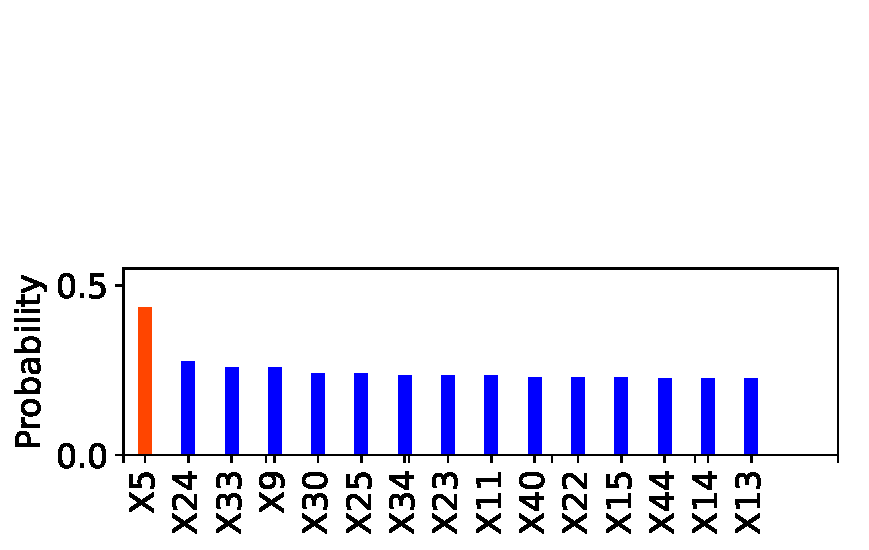
\includegraphics[width=0.25\paperwidth]{acc_plot_top20_ic_5_False_lars-crop.pdf}}

  \subfloat[\label{fig:solar_ic_type-II7}$\omega = 1/4,\;\mu\left(F\right)=1/2$, solar]
  {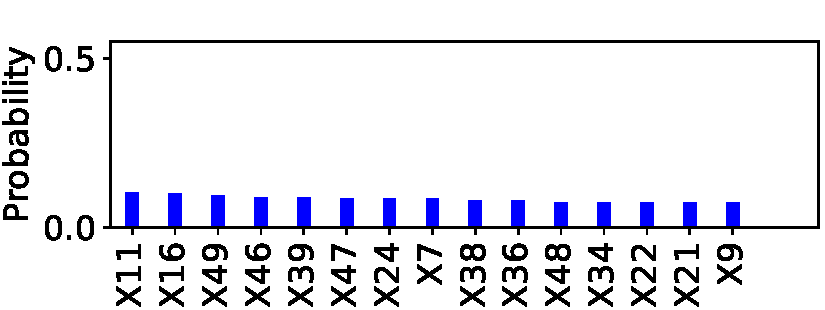
\includegraphics[width=0.25\paperwidth]{acc_plot_top20_ic_25_False_solar-crop.pdf}}
  %
  \subfloat[\label{fig:solar_ic_type-II8}$\omega = 1/3,\;\mu\left(F\right)=2/3$, solar]
  {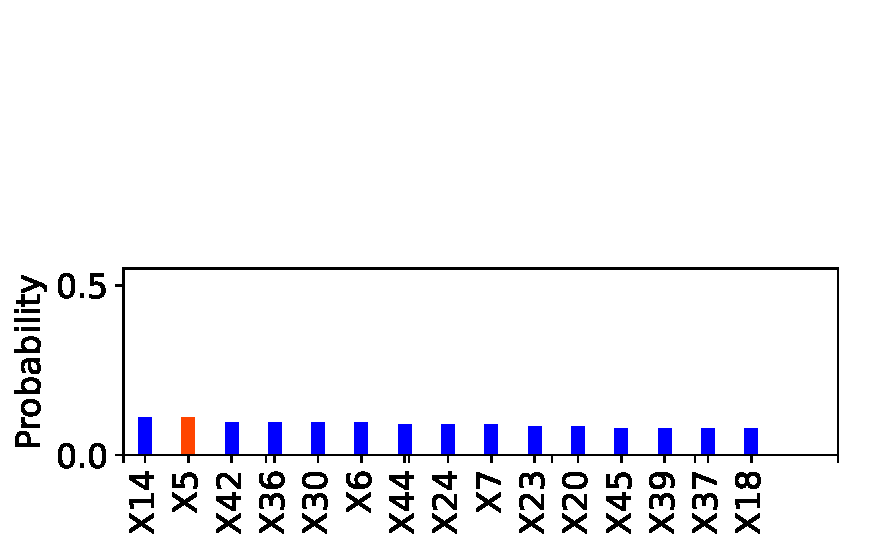
\includegraphics[width=0.25\paperwidth]{acc_plot_top20_ic_33_False_solar-crop.pdf}}
  %
  \subfloat[\label{fig:solar_ic_type-II9}$\omega = 1/2,\;\mu\left(F\right)=1$, solar]
  {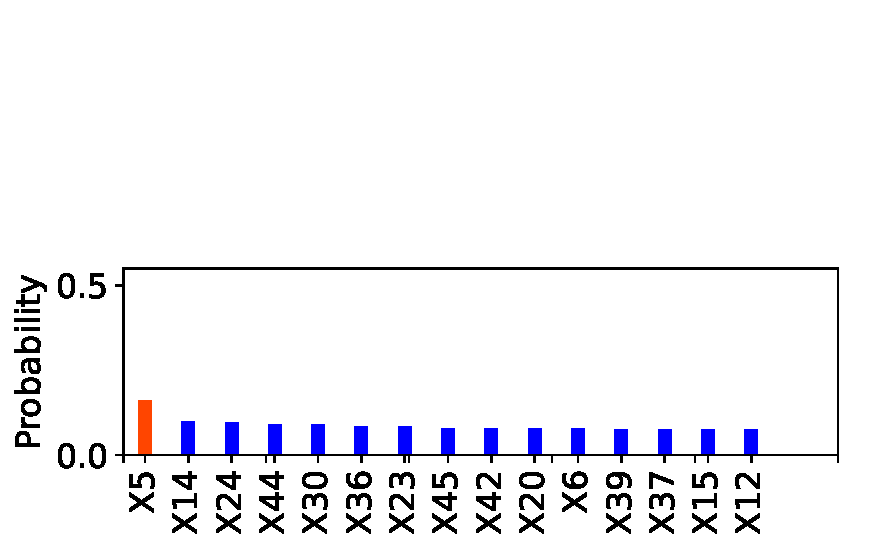
\includegraphics[width=0.25\paperwidth]{acc_plot_top20_ic_5_False_solar-crop.pdf}}
  %
  \caption{Probability of including redundant variables (top 15) in simulation~2 ($\mathbf{x}_5$ in orange).}
  \label{fig:solar_ic_type-II}
  %
\end{figure}

In (\ref{eqn:dgp_x5}), IRC only affects the redundant $\mathbf{x}_5$. Hence, we focus on the probability of wrongly selecting $\mathbf{x}_5$ over 200 repetitions. By setting $\omega$ to either $1/4$, $1/3$, or $1/2$, the population value of $\mu \left( F \right)$ changes, respectively, to $1/2$, $2/3$, or $1$, gradually increasing the difficulty of purging the redundant $\mathbf{x}_5$. Figure~\ref{fig:solar_ic_type-II} displays the simulation results. When $\mu \left( F \right) = 1/2$, lasso wrongly includes $\mathbf{x}_5$ with probability $0.25$. By contrast, $\mathbf{x}_5$ does not crack the top-10 list for solar, implying that the corresponding probability remains below $0.1$. When $\mu \left( F \right)$ increases to $2/3$, the probability that lasso includes $\mathbf{x}_5$ increases to around $0.3$, standing out from the other 9 variables. When $\mu \left( F \right)$ jumps to $1$ in the population and strong IRC is violated, the probability that lasso includes $\mathbf{x}_5$ rises to almost $0.5$. Despite the increase in $\mu\left(F\right)$, the probability that solar includes $\mathbf{x}_5$ is always below $0.1$. The results illustrate that solar is more robust to different settings of the IRC.


%%%%%%%%%%%%%%%%%%%%%%%
%%%%%% SECTION 4 %%%%%%
%%%%%%%%%%%%%%%%%%%%%%%

\section{Solar improvements over lasso-related, subsampling variable selection\label{section:comp}}

In this section, we show that: (i) solar and hold-out averaging offer significant improvements over lasso-type algorithms in terms of variable selection sparsity, stability, accuracy, and; (ii) replacing lasso with solar in subsampling variable selection drastically reduces the computational load (both runtime and subsample repetition) while improving sparsity and accuracy.

\subsection{Simulation competitors}

We do not consider all lasso-type algorithms for comparison. Firstly, some lasso modifications (e.g., fused lasso, grouped lasso) are designed to solve specific empirical problems that are not relevant to our paper. Secondly, it may be difficult to determine how much some variants outperform lasso.\footnote{For example, while \citet{jia2010model} show numerically that elastic net has slightly better variable-selection accuracy than lasso, they also find that ``when the lasso does not select the true model, it is more likely that the elastic net does not select the true model either'' (a point we verify in Section~\ref{section:application}). While simulations in \citet{zou2006adaptive} show that adaptive lasso outperforms lasso when $p/n<1$, it requires first computing the OLS estimates of all $\mathbf{x}_i$ coefficients, which is difficult when $p/n>1$.} Since both solar and lasso may be evaluated via least-angle regression and coordinate descent, many other lasso modifications can be directly applied to solar, as discussed in section~3.1. We also do not consider information criteria for shrinkage parameter tuning. \citet{scikit-learn} points out that information criteria are over-optimistic and require a proper estimation of the degrees of freedom of the solution. Moreover, information criteria are derived asymptotically and tend to breakdown when the problem is badly conditioned (e.g., $p > n$).\footnote{See \url{https://scikit-learn.org/stable/modules/linear_model\#lasso.html} for details.}

Least-angle regression and coordinate descent yield nearly identical selection results for solar and lasso. Hence, we combine the lars results and coordinate descent results for solar, ignore the coordinate descent lasso (which is included in the supplementary files), and report only the runtime comparison between least-angle regression and coordinate descent.

Along with lasso, we include subsampling variable selection algorithms (aka subsampling ensembles). A lasso subsampling ensemble repeats lasso multiple times across subsamples, producing the averaged (or accumulated) selection result of the repetitions. In our simulation, we compare the lasso and solar subsampling ensembles and demonstrate that the solar ensemble improves variable selection performance and substantially reduces computation load. Due to the similarity across lasso subsampling ensembles, we choose the bootstrap lasso \citep{bach2008bolasso} to be the competitor. \citet{bach2008bolasso} proposes two bolasso algorithms: bolasso-H and bolasso-S. Bolasso-H selects only variables that are selected in all subsamples, i.e., the subsample selection frequency threshold, $f=1$. Bolasso-S selects variables that are selected in 90\% of the subsamples ($f=0.9$). In our simulation, we use both as the competitors. \citet{bach2008bolasso} finds that it is always beneficial, in terms of selection and prediction, to generate more subsamples in bolasso. Hence, to compare solar with state-of-art bolasso performance, we set the number of subsamples in bolasso to $256$, the maximum in the \citet{bach2008bolasso} simulations.

In a similar vein, we introduce the bootstrap solar ensemble \emph{(bsolar)}, which runs solar on each subsample and computes the selection frequency for each variable across subsamples. To ensure that any performance improvement is due to replacing lasso with solar in the ensemble system, bsolar and bolasso use the same $f$. Thus, we evaluate 2~versions of bsolar: bsolar-H ($f=1$) and bsolar-S ($f=0.9$). To denote the number of subsamples clearly, we use the notation bsolar-$m$H and bsolar-$m$S, where $m$ is the number of subsamples used to compute the selection frequency.

\subsection{Simulation settings}

The DGP is as follows. \hl{All $p$ covariates in $X \in \mathbb{R}^{n \times p}$ are generated by a zero-mean, multivariate Gaussian, where the covariance matrix has 0.5~for all the off-diagonal elements. The first 5 variables are informative and the remaining $p-5$ variables are redundant. Thus, the response variable $Y \in \mathbb{R}^{n \times 1}$ is given}
%
\begin{equation}
%
  Y =  2 \mathbf{x}_0 + 3 \mathbf{x}_1 + 4 \mathbf{x}_2 + 5 \mathbf{x}_3 + 6 \mathbf{x}_4  + e,
  \label{eqn:pop_model}
\end{equation}
%
\hl{where $e\in \mathbb{R}^{n \times 1}$ is a standard Gaussian noise term.} All data points are independently and identically distributed. Each $\mathbf{x}_j$ is independent from the noise term $e$, which is standard Gaussian. Solar competes with $K$-fold, cross-validated lasso (denoted `lasso' for short). We choose the number of CV folds and the number of subsamples generated in Algorithm~\ref{algo:APE-lar} to be $10$, following the \citet{friedman2001elements} simulations that show $K = 10$ balances the bias-variance trade-off in CV error minimization.

We use three criteria to compare the variable-selection performance of solar and lasso: sparsity, accuracy, and runtime. Sparsity is measured by the mean of the number of variables selected. Accuracy is measured by the average number of selected informative variables. Runtime is the average CPU time for one realization.

In this simulation, we generate data with various $p/n$ (each with 200 repeats and fixed Python random generators) as follows. In scenario 1, $p/n$ approaches $0$ from above, corresponding to the classical $p<n$ setting. In scenario 2, $p/n$ approaches $1$ from above, corresponding to high-dimensional settings. In scenario 3, $p/n=2$ as $\log(p)/n$ slowly approaches $0$, corresponding to ultrahigh-dimensional settings, i.e., where $(p-n)\rightarrow\infty$. The raw simulation results are also in the supplementary file.

\subsection{Programming languages, parallelization and hardware for simulations}

We carefully design the simulation settings so that our comparisons are fair, representative, and generalizable and, in particular, to enable a like-for-like comparison to state-of-the-art lasso algorithms.

First, to maximize computation speed, we use \texttt{Numpy}, \texttt{Scipy}, and \texttt{Cython}---all well-known for performance and speed---to outsource all numerical and matrix operations to \texttt{Intel MKL}, currently the fastest and most accurate C++/Fortran library for CPU numerical operations.

Second, to reduce the possibility of CPU and RAM bottlenecks in parallel computing of the lasso and lasso-related subsampling algorithms, we choose Python rather than R as the programming interface. Research shows [e.g., \citet{donoho201750}]  that ``R has the well-known reputation of being less scalable than Python to large problem sizes'', which is  due to its memory-CPU management. Given the simulations repeat solar, lasso, and lasso-related subsampling algorithms many times to arrive at accurate average performance measures, choosing Python over R greatly reduces any potential hardware limitations. Moreover, computations are carried out with an Intel Xeon W-3245 CPU with 3.2GHz frequency, 10-processor parallelization, and 64GB RAM, further reducing the possibility of CPU-RAM bottlenecks.

Third, to guarantee the programming quality of the lasso package, we implement lasso and lasso-related subsampling algorithms from the {\sf Sci-kit learn} library \citep{scikit-learn}, one of the most efficient machine-learning packages and one that is widely used in research and industry.\footnote{More detail is available at \url{https://scikit-learn.org/stable/}.} {\sf Sci-kit learn} also use \texttt{Numpy}, \texttt{Scipy} and \texttt{Cython} to source all numerical/matrix operations to the Fortran/C++. Again, the idea is to maximize the lasso computation speed.

Lastly, to optimize computation and avoid large overheads, we implement 10-processor parallelization. Because each realization of solar and CV-lasso requires 10 repetitions of lars or pathwise coordinate descent, optimization must be carried out sequentially, meaning that each realization of solar or lasso must wait for the preceding realization to finish. Thus, we design the parallel architecture to assign one realization per CPU core. The design is optimized for a CPU with at least 10 cores and may generate a parallel overhead with fewer cores. For example, in each realization, an 8-core CPU would assign two cores to training the second repetition of coordinate descent with the other 6 remaining idle until all 10 repetitions are finished.

\subsection{Accuracy and sparsity comparison with varying p/n \label{subsection:suml1}}

\begin{table}[h]
%
%\small
\centering
%
\caption{Simulation result.\label{table:sim_1}}
\smallskip
%
\resizebox{0.98\textwidth}{!}{%
\renewcommand{\arraystretch}{0.7}
\begin{tabular}{ll.........}
  \toprule
        &
        & \multicolumn{3}{c}{$p/n\rightarrow0$}
        & \multicolumn{3}{c}{$p/n\rightarrow1$}
        & \multicolumn{3}{c}{$\log(p)/n\rightarrow0$} \\
        \cmidrule(lr){3-5} \cmidrule(lr){6-8} \cmidrule(lr){9-11}
        &                              & \multicolumn{1}{c}{$\frac{100}{100}$} & \multicolumn{1}{c}{$\frac{100}{150}$} & \multicolumn{1}{c}{$\frac{100}{200}$} & \multicolumn{1}{c}{$\frac{150}{100}$} & \multicolumn{1}{c}{$\frac{200}{150}$} & \multicolumn{1}{c}{$\frac{250}{200}$} & \multicolumn{1}{c}{$\frac{400}{200}$} & \multicolumn{1}{c}{$\frac{800}{400}$} & \multicolumn{1}{c}{$\frac{1200}{600}$}  \\
  \midrule
  average number of  & lasso            & 19.73 & 19.84 & 19.54 & 22.30 & 23.57 & 26.56 & 28.92 & 33.88 & 37.96 \\
  selected variables & solar            &  9.86 &  8.66 &  8.50 & 11.34 &  9.8  &  8.2  & 10.54 & 13.28 & 15.52 \\
                     & solar + hold out &  5.02 &  5.12 &  5.17 &  4.99 &  5.16 &  5.13 &  5.12 &  5.24 &  5.26 \\
                     \\ [-8pt]

                     & bsolar-3S/3H     & 5.44  & 5.18  & 5.22  & 5.44  & 5.18  & 5.22  & 5.25  & 5.86  & 6.09  \\
                     & bsolar-5S/5H     & 5.14  & 5.07  & 5.1   & 5.14  & 5.07  & 5.1   & 5.08  & 5.28  & 5.46  \\
	                   & bsolar-10S       & 5.12  & 5.04  & 5.04  & 5.12  & 5.04  & 5.04  & 5.05  & 5.24  & 5.39  \\
                     & bsolar-10H       & 5.06  & 5.01  & 5     & 5.06  & 5.01  & 5     & 5.01  & 5.09  & 5.17  \\
                     \\ [-8pt]

	                   & bolasso-S        & 5.46  & 6.09  & 6.60  & 5.46  & 6.09  & 6.6   & 5.58  & 6.63  & 7.67  \\
	                   & bolasso-H        & 5     & 5.02  & 5.01  & 5     & 5.02  & 5.01  & 5     & 5.01  & 5.02  \\
  \\[-8pt]
  average number of    & lasso            & 5    & 5 & 5 & 5    & 5 & 5 & 5 & 5 & 5 \\
  selected informative & solar            & 5    & 5 & 5 & 5    & 5 & 5 & 5 & 5 & 5 \\
  variables            & solar + hold out & 4.95 & 5 & 5 & 4.91 & 5 & 5 & 5 & 5 & 5 \\

  \\ [-8pt]
                       & bsolar-3S/3H/5S/5H/10S/10H & 5 & 5 & 5 & 5 & 5 & 5 & 5 & 5 & 5 \\

                       \\ [-8pt]
	                     & bolasso-S/H      & 5 & 5 & 5 & 5 & 5 & 5 & 5 & 5 & 5 \\
  \\[-8pt]
  average runtime & solar + hold out       & 0.07  & 0.08  & 0.08  & 0.08  & 0.10  & 0.13  & 0.19  & 0.49   & 0.83   \\
                  & bsolar-3               & 0.11  & 0.16  & 0.15  & 0.10  & 0.15  & 0.22  & 0.41  & 0.74   & 1.48   \\
                  & bolasso (lars, 256 SR) & 9.52  & 12.49 & 10.61 & 10.01 & 13.92 & 19.72 & 23.10 & 184.59 & 502.56 \\
                  & bolasso (cd,   256 SR) & 13.49 & 60.51 & 60.35 & 13.92 & 16.85 & 20.17 & 27.73 & 100.58 & 308.12 \\
  \bottomrule
  \end{tabular}}
  %
\end{table}

Table~\ref{table:sim_1} summarizes the average selection performance.\footnote{Detailed histograms are in the supplementary file.} While solar and lasso always include all 5 informative variables, solar clearly outperforms lasso in terms of sparsity in every $p/n$ scenario, implying a much better ability to control redunant variable inclusion. More interestingly, the lasso sparsity deteriorates as $p/n$ approaches $1$, while solar sparsity continues to improve. As $\log(p)/n\rightarrow0$, while the sparsity of each competitor deteriorates, solar maintains a clear advantage over lasso.

Table~\ref{table:sim_1} also confirms a solar advantage over lasso in subsampling ensembles. All subsampling ensembles select the $5$ informative variable with probability $1$. Among all subsampling ensembles, bolasso-S sparsity is always the worst while the others perform nearly identically. However, bolasso requires 256 subsample lasso repetitions while bsolar-3, -5 and -10 only take 3, 5, and 10 subsample solar repetitions, respectively. Hence, bsolar reduces  subsample repetitions by 96\%. \hl{As we show in Section}~\ref{subsection:comp}\hl{, solar and lasso have identical computation loads. As a result, the 96\% reduction in subsample repetitions implies at least a 96\% reduction in computation time, assuming time complexity increases linearly.}

Most importantly, the performance of \emph{solar $+$ hold out} (the combination of solar and the hold-out average) in Table~\ref{table:sim_1} illustrates that solar performance can be further boosted by hold-out average test. Provided $n$ is not very small (a necessary requirement for hypothesis testing), \emph{solar $+$ hold out} sparsity and accuracy are on par with any subsampling variable selection method. It is worth noting that, with limited degrees of freedom (fewer than 50 when $n=100$), \emph{solar $+$ hold out} occasionally omits informative variables. Under such a situation, bsolar, which has a similar computation time, would be a better choice. Overall, these results confirm and supplement the Example~1 findings.

\subsection{Bolasso-bsolar efficiency discrepancy and explanations}

\hl{Most lasso-related subsampling selection algorithms require completing CV-lasso on each subsample, multiplying the computation load despite ranking the variables only once. However, bsolar performs similar to bolasso with only 4\% of the 256 subsample repetitions required by bolasso.} The efficiency of bsolar is due to its unique \emph{multi-layer variable ranking scheme}.

\begin{itemize}
  \item Algorithms~\ref{algo:APE-lar} and \ref{algo:APE-cd} show that solar internalizes a variable ranking scheme (the \emph{internal ranking}) without increasing the computational burden above lasso (see section~\ref{subsection:comp}). Internal ranking significantly improves variable selection performance.

  \item Bsolar further embeds solar into a bootstrap ranking framework. That is, once solar has ranked and selected variables on each subsample, bsolar collects the highly ranked variables across the subsamples and produces a ranking based on new test data, selecting the most stable of the strong signals (the \emph{external ranking}).
\end{itemize}

\noindent
Research (\citet{fan2008sure, hall2009usingb, hall2009using, li2012robust, li2012feature}) confirms the efficiency of one-layer ranking. \hl{Thus, the efficiency of multi-layer ranking is not surprising.}

\begin{table}[!htb]
  \caption{Subsample selection frequency for bolasso and bsolar-10.}
  \label{table:subsample_select_freq}
  \begin{minipage}[t]{.56\linewidth}
    \small
    \subfloat[bolasso]{%
    \label{table:subsample_select_freq_1}
			\renewcommand{\arraystretch}{0.7}
			\begin{tabular}{cl}
				\toprule
				frequency & variables \\
				\midrule
				$\geqslant 1.00$ & $\mathbf{x}_4, \mathbf{x}_3, \mathbf{x}_2, \mathbf{x}_1, \mathbf{x}_0$ \\
				$\geqslant 0.88$ & $\mathbf{x}_4, \mathbf{x}_3, \mathbf{x}_2, \mathbf{x}_1, \mathbf{x}_0, \mathbf{x}_{28}$ \\
				$\geqslant 0.84$ & $\mathbf{x}_4, \mathbf{x}_3, \mathbf{x}_2, \mathbf{x}_1, \mathbf{x}_0, \mathbf{x}_{28}, \mathbf{x}_{71}$\\
				$\geqslant 0.76$ & $\mathbf{x}_4, \mathbf{x}_3, \mathbf{x}_2, \mathbf{x}_1, \mathbf{x}_0, \mathbf{x}_{28}, \mathbf{x}_{71}, \mathbf{x}_{91}$\\
				$\geqslant 0.70$ & $\mathbf{x}_4, \mathbf{x}_3, \mathbf{x}_2, \mathbf{x}_1, \mathbf{x}_0, \mathbf{x}_{28}, \mathbf{x}_{71}, \mathbf{x}_{91}, \mathbf{x}_{94}$\\
				$\geqslant 0.69$ & $\mathbf{x}_4, \mathbf{x}_3, \mathbf{x}_2, \mathbf{x}_1, \mathbf{x}_0, \mathbf{x}_{28}, \mathbf{x}_{71}, \mathbf{x}_{91}, \mathbf{x}_{94}, \mathbf{x}_{70}, \mathbf{x}_{40}$ \\
        $\vdots$ & $\vdots$ \\
				\bottomrule
		\end{tabular}}
  \end{minipage}
  \begin{minipage}[t]{.5\linewidth}
    \small
    \subfloat[bsolar-10]{%
    \label{table:subsample_select_freq_2}
			\renewcommand{\arraystretch}{0.7}
			\begin{tabular}{cl}
				\toprule
				frequency & variables \\
				\midrule
				$\geqslant 1.00$ & $\mathbf{x}_4, \mathbf{x}_3, \mathbf{x}_2, \mathbf{x}_1, \mathbf{x}_0$ \\
				$\geqslant 0.10$ & $\mathbf{x}_4, \mathbf{x}_3, \mathbf{x}_2, \mathbf{x}_1, \mathbf{x}_0, \mathbf{x}_{91}, \mathbf{x}_{71}$ \\
				\bottomrule
		\end{tabular}
    }
  \end{minipage}
\end{table}

Table~\ref{table:subsample_select_freq} shows numerically how efficient multi-layer ranking is. Table~\ref{table:subsample_select_freq_1} breaks down the subsample selection frequency list from 256 subsamples for one bolasso realization with $p/n=100/200$. Due to the length of the list, we report only subsample selection frequencies $\ge0.69$. With only one layer of ranking, bolasso is unable to separate informative from redundant variables even with 256 subsample repetitions. The frequency discrepancy for bolasso between the highest-ranking redundant ($\mathbf{x}_{28}$) and the lowest-ranking informative variable ($\mathbf{x}_0$) is only $0.12$. By contrast, bsolar-10 returns a much shorter list and the frequency discrepancy between the highest-ranking redundant ($\mathbf{x}_{91}$) and the lowest-ranking informative variable ($\mathbf{x}_0$) is $0.9$. To increase the discrepancy between the lowest ranked informative and highest ranked redundant variables for bolasso, \citet{bach2008bolasso} suggests raising the number of subsample repetitions. However, increasing repetitions further raises the bolasso computation load in high-dimensional spaces, making bsolar even more preferable.

\subsection{Computation load comparison \label{subsection:comp}}

Since the computation load for lars or coordinate descent on a given sample is fixed, we may use the number of lars or coordinate descents to approximate the computation loads of solar and lasso. For comparison, we compute solar with $K$ subsamples and lasso with $K$-fold cross-validation. As shown in Algorithm~\ref{algo:APE-lar} and \ref{algo:APE-cd}, solar computes one lars or coordinate descent on each subsample $(X^k, Y^k)$, implying it needs to estimate $K$ lars or coordinate descents to compute $\widehat{q}$ and one more to compute $c^*$ for variable selection. Lasso also requires computing $K$ lars or coordinate descents to optimize the tuning parameter and, given the optimal tuning parameter, one more on the full sample to select variables. Thus, solar and lasso have the same computation load.

Given computation load equality for solar and lasso, differences between bolasso and bsolar are due primarily to the number of subsample repetitions (SR). Thus, solar and lasso have a computation load of $1$ SR, bolasso has a load of $256$ SR, and bsolar-3/5/10 each has a load of $3/5/10$ SR.

Since bsolar and bolasso have very similar computation procedures, they are coded similarly to make any comparison fair. \hl{The main code difference lies in computing the subsample selection frequency.}\footnote{See \texttt{README.html} in the supplementary file for more detail.} \hl{Thus, runtime differences below are due to the reduction in subsample repetitions from the solar ensemble.} To maximize bolasso computation speed, we use the built-in \texttt{Sci-kit learn} parallel scheme \hl{(denoted as \emph{built-in parallel})}, which is fully optimized for lasso. Following the recommendation of \texttt{Sci-kit learn}, we design a high-performance parallel architecture for \emph{solar + hold out} and bsolar.

Table~\ref{table:sim_1} summarizes average runtime for 10 repetitions on an Intel Xeon W-3245 CPU with 3.2GHz frequency, 10-processor parallelization, and 64GB RAM. Both \emph{solar + hold out} and bsolar-3 have much shorter runtimes than bolasso. The runtime differences are even more pronounced when $p$ and $n$ increase. \hl{The 256 subsample repetitions render the bolasso variable selection algorithms computationally infeasible even with moderate $p$ and $n$.} By contrast, bsolar-3 requires only 30 realizations of lars or coordinate descent. Due to a lighter computational load and CPU usage, bsolar-3 allows the CPU to work at a higher frequency than for bolasso, decreasing the runtime for each lars realization.

\subsubsection{Comparison with previous lasso computation research}

The bolasso findings are consistent with previous research on lasso. \hl{Given the same  convergence criteria (the tolerance for the optimzation and the maximum number of iterations), number of folds for CV ($K=10$), and number of $\lambda$s in the grid search (100), the time complexity of lasso is mostly relevant to $n$, $p$, and pairwise correlation among the covariates ($corr$)}. Thus, we conduct the following comparisons for the Gaussian regression with $p/n=1000/100$ and $corr=0.5$.

\begin{itemize}
  %
  \item \citet[Table 1]{friedman2010regularization} shows that, on a 2-core Intel Xeon CPU with 2.8GHz frequency, the average runtime of one pathwise coordinate descent realiztion in Fortran is 0.07 seconds with covariance precomputed for updating. The \citet{friedman2010regularization} result only record the time for coordinate descent computation.
  %
  \item Using Intel Xeon W-3245 CPU with 3.2GHz frequency and 10-processor parallelization, the average runtime for our coordinate descent bolasso package is 41.92 seconds with covariance precomputed automatically, accounting for 256 realizations of 10-fold, cross-validated lasso. Hence, the total 41.92 seconds is for 2816 coordinate descent realizations, resulting in 0.014 seconds per realization. 
  %
\end{itemize}

Comparing our results to \citet{friedman2010regularization}, the average speedup for one pathwise coordinate descent is roughly 5. \hl{With the same computataion amount,} the theoretical maximum speedup may be accurately calculated using Amdahl's law. Both lars and coordinate descent require 10 repetitions to optimize $\lambda$ and one to compute $\beta$, implying that 1 of the 11 repetitions (11\% of the computations, including data generation, variable ranking, matrix manipulation, I/O, etc.) is not parallelizable. With a given computation load ($n$ and $p$), Amdahl's law implies that the 16-core maximum speedup over 2-core is roughly
%
\begin{equation}
  %
  \frac{1}{\rho + (1-\rho)/s} = \frac{1}{0.11 + (1-0.11)/(16/2)} \approx 4.52.
  %
\end{equation}
%
\hl{where $\rho$ is the proportion of computation that is not parallelizable and $s$ is the computation speedup for the parallelizable proportion (e.g., the core number multiple).\footnote{see \url{https://en.wikipedia.org/wiki/Amdahl's_law} for a brief introduction.} Given that our CPU frequency is also higher than} \citet[Table 1]{friedman2010regularization} \hl{($3.2$GHz over $2.8$), we adjust the maximum speedup by the frequency multiple ($3.2/2.8$), resulting in a final maximum speedup of $4.52 \times 3.2/2.8 \approx 5.17$.}

\begin{figure}[h]
  %
  \centering
  %
  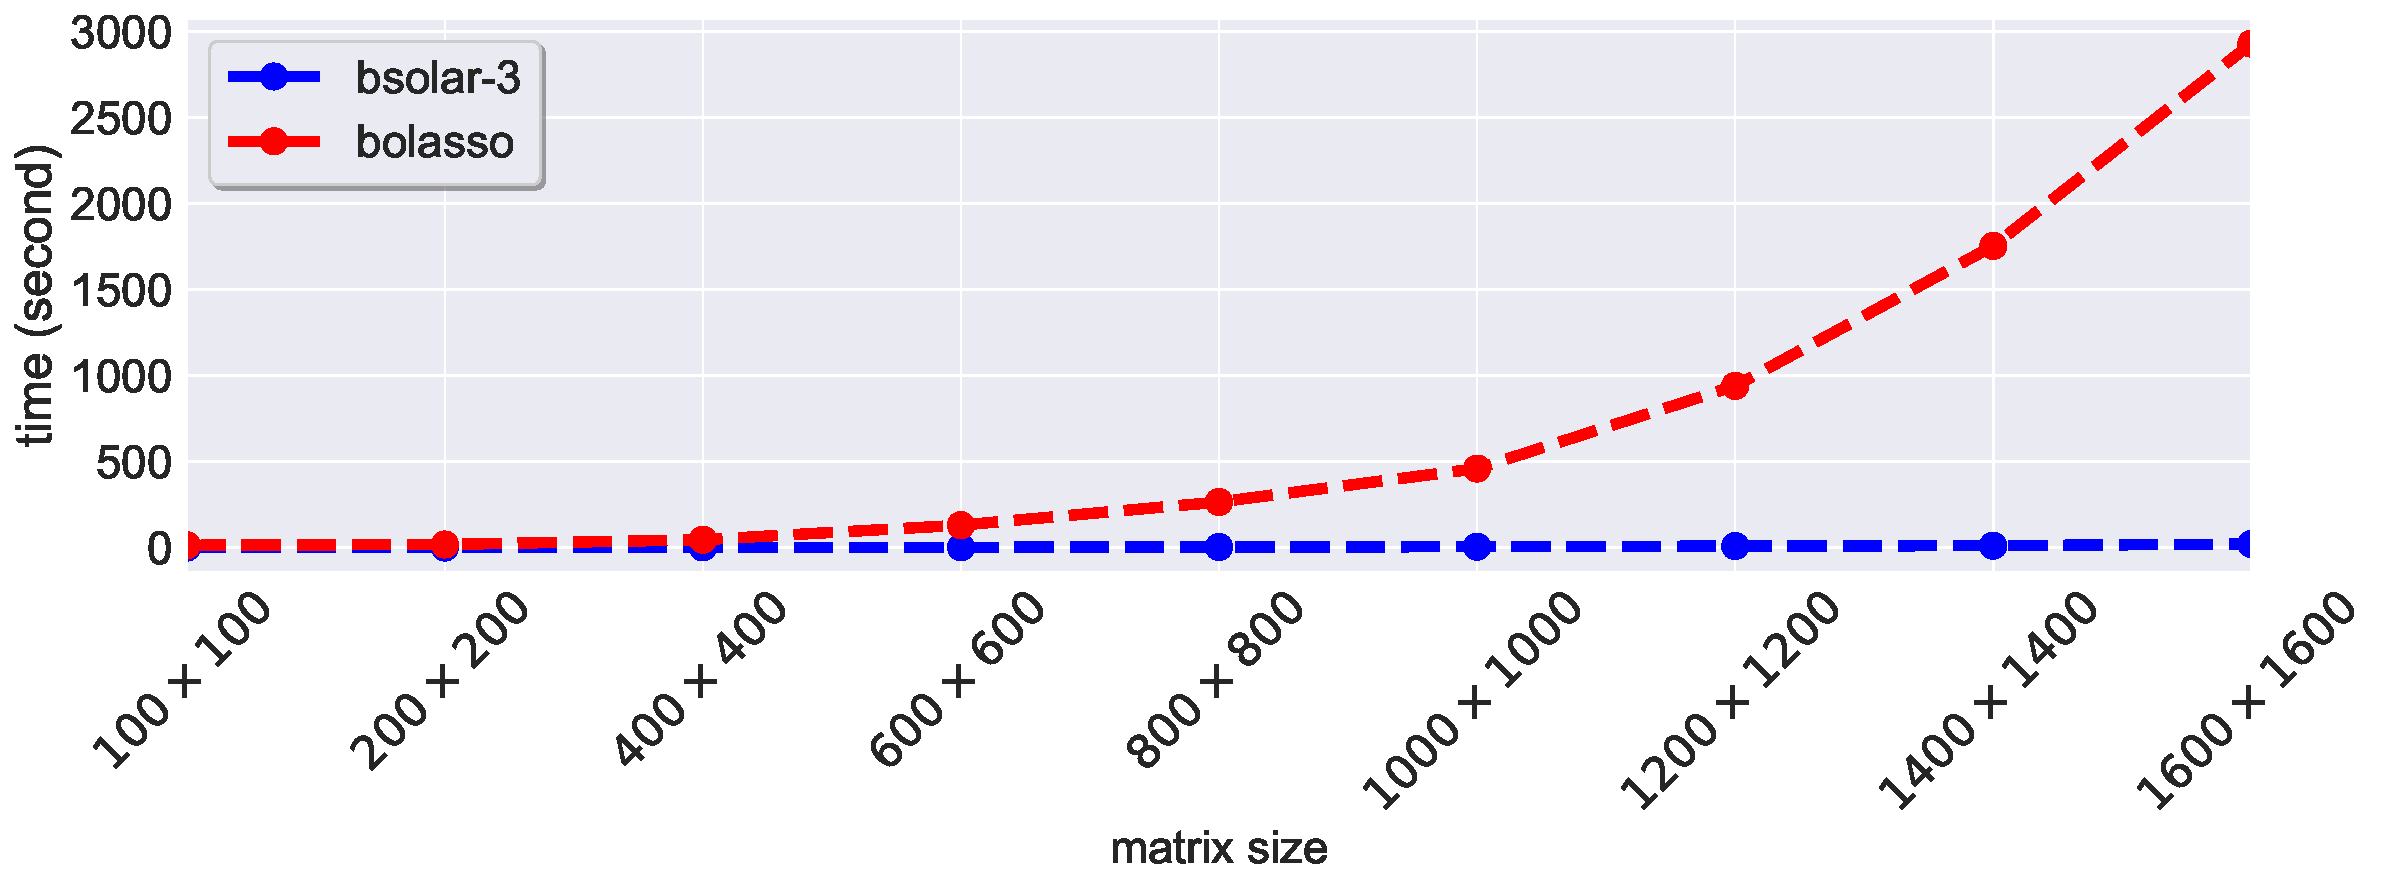
\includegraphics[width=0.8\linewidth]{runtime.pdf}
  %
  \caption{Average runtime comparison with different input matrix sizes (by pathwise coordinate descent).}
  %
  \label{fig:runtime}
  %
\end{figure}


\hl{It is difficult to make a perfectly fair comparison of runtimes with different hardware. However, benchmarking the parallel computation efficiency of the lasso speedup with Amdahl's law, the coordinate descent bolasso package appears to be very competitive.} Nonetheless, bolasso still requires a large computation time with $p/n=1200/600$ due to the $256$ CV-lasso repetitions, once again confirming the bsolar computation advantage. Figure~\ref{fig:runtime} \hl{shows how average runtime changes as the input matrix size increases. Regression algorithms in reproducing kernel Hilbert spaces (e.g., the kernel ridge and kernel lasso regression) use kernel tricks to transform the data matrix $X\in\mathbf{R}^{n\times p}$ into an input matrix $F \in \mathbf{R}^{n\times n}$ and optimize over $F$. Thus, matrix size in} Figure~\ref{fig:runtime} \hl{emulates how computation load increases for bootstrap kernel lasso. As matrix size increases, bsolar runtime increase remains linear while bolasso rises exponentially, confirming the bsolar-3 advantage for large input matrices.}

Due to the lean parallelization design, the solar parallelization can be further improved. However, for a fair bsolar-bolasso comparison, we design the 10-processor parallelization algorithm to be the same for both. Due to the small number of subsample solar repetitions (3), our 10-processor parallelization is more than sufficient for bsolar-3. Thus, unlike bolasso, the performance of bsolar will not be compromised by the number of CPU cores, implying a similar efficiency on 4- and 8-core CPUs (such as i7-8500u and i9-9900k). By contrast, bolasso will suffer a large parallel overhead with a smaller number of CPU cores due to its large computation load.

The runtime analysis may be extended to a comparison between the hold-out average and the bootstrap-based data-splitting tests, as in \citet{meinshausen2009p}. Bootstrap-based data-splitting tests require computationally costly, bootstrap-like repetitions: each bootstrap subsample is split, with one portion used for selection and the other for testing. Thus, with lasso used for variable selection, the runtime for the bootstrap-based data-splitting test with 256 bootstrap subsamples will be close to that of bolasso in Table~\ref{table:sim_1}. By contrast, the hold-out average only uses one realization of variable selection and two t-tests, offering a faster runtime.

\section{Real-world data: Sydney house price prediction\label{section:application}}

To demonstrate that the improvements from solar are empirically feasible, we apply solar to real-world data. In the context of the simulations above, the real-world data reflect both the $p/n\rightarrow0$ scenarios of simulation~1 and the high multicollinearity and complicated dependence structures of simulation~2. As such, the data reflect the challenging IRC settings, complicated dependence structures, and grouping effects typical of data in the social sciences.

The sample is assembled from more than 10 different databases: Sydney, Australia, real estate market transaction data for 11,974 houses sold in 2010, including price and house attribute information (property address, bedrooms, bathrooms, car spaces, etc.), matched to 2011 census data by Statistical Area Level 1 (the smallest census area in Australia, comprising at most 200 people or 60 households), 2010 and 2011 crime data by suburb, 2010 GIS data (extracted from a geo-spatial topological database, a climate database, a pollution database, and the Google Maps database), 2009 primary and secondary school data, and 2010 Sydney traffic and public transport data (bus routes, train stations, and ferry wharfs). We predict house price with a linear model.

Using an ensemble of Bayes network learning algorithms for data clearning, we purge variables with both very low conditional and unconditional correlations to house price. The remaining variables are listed in the first column of Table~\ref{table:house_variable}.\footnote{Due to 200GB size of the database, we only include the data for these variables in the supplementary file.} The 57 variables fall into 5 categories: house attributes, distance to key locations (public transport, shopping, etc.), neighbourhood socio-economic data, localized administrative and crime data, and local school quality. Pairwise correlations among all 57 covariates indicate, not surprisingly, severe multicollinearity and grouping effects, implying a harsh IRC setting.\footnote{Correlations and IRC are also reported in supplementary files.} Thus, heuristically increasing the value of the tuning parameter in lasso-type estimators (e.g., using the one-sd or the `elbow' rule) is unlikely to be useful since it may trigger further grouping effects and the random dropping of variables.

Table~\ref{table:house_variable} shows the selection comparison across the elastic net, lasso, and solar. With all variables in linear form, both lasso and elastic net lose sparsity due to the complicated dependence structures and severe multicollinearity in the data, consistent with \citet{jia2010model}. By contrast, solar returns a much sparser model, with only $9$ variables selected from $57$. A very similar result can be found with the variables in log form, hinting that solar possesses superior selection sparsity and robustness to a change in functional form. More importantly, solar variable selection outperforms the lasso-type estimators in terms of the balance between sparsity and prediction power. While pruning most of the variables from the elastic net and lasso selections, solar reduces the post-selection regression $\mathrm{R}^2$ by only 3-5\%. In the supplementary file, we also perform a hold-out average method to avoid the possibility that the `p-value overfitting' issue also affects the direct post-selection OLS $R^2$. However, there is no concern in this sample because $p/n=57/11,974$. This confirms that, from the perspective of prediction, solar successfully identifies the most important variables in the database.

%%%%%%%%%%%%%%%%%%%%%%%%%%%%%%%%%%
%%%%%%%%%%% Conclusion %%%%%%%%%%%
%%%%%%%%%%%%%%%%%%%%%%%%%%%%%%%%%%

\section{Conclusion}

In this paper we offer a new least-angle regression algorithm for high-dimensional data called solar (for subsample-ordered least-angle regression). We show that solar yields substantial improvements over lasso in terms of the sparsity, stability, accuracy, and robustness of variable selection. We also illustrate the improvements relative to lasso ensembles from solar ensembles in terms of variable selection accuracy, sparsity and computation load.

Detection of weak signals is a small weakness evident in solar, although relative to the lasso competitor the difference is very slight. Nonetheless, we are working on an extension to solar, the double-bootstrap solar (DBsolar), which, if early results are any indication, promises to enable solar accurately to detect variables with weak signals.

%%%%%%%%%%%%%%%%%%%%%%%%%%%%%%%%%%
%%%%%%%%%%% References %%%%%%%%%%%
%%%%%%%%%%%%%%%%%%%%%%%%%%%%%%%%%%

\bibliographystyle{elsarticle-harv}
%\bibliographystyle{CJE}

\bibliography{ref/CVrefs}

\begin{table}[H]
  %
  \centering
  %
  \small
  %
  \caption{Variable selection results for linear and log house price models. \label{table:house_variable}}
  %
  \resizebox*{!}{0.95\textheight}{%
  \renewcommand{\arraystretch}{0.6}
  \begin{tabular}{@{}ll@{\extracolsep{6pt}}c@{\extracolsep{-2pt}}c@{\extracolsep{6pt}}c@{\extracolsep{-2pt}}c@{\extracolsep{6pt}}c@{\extracolsep{-2pt}}c@{}}
    %
    \toprule
    %
            &             & \multicolumn{2}{c}{elastic net}
                          & \multicolumn{2}{c}{lasso}
                          & \multicolumn{2}{c}{solar} \\
                          \cline{3-4} \cline{5-6} \cline{7-8} \\[-7pt]
    %
    Variable & Description& \multicolumn{1}{c}{linear}
                          & \multicolumn{1}{c}{log}
                          & \multicolumn{1}{c}{linear}
                          & \multicolumn{1}{c}{log}
                          & \multicolumn{1}{c}{linear}
                          & \multicolumn{1}{c}{log} \\
    %
    \midrule
    %
    Bedrooms           & property, number of bedrooms             & \checkmark  & \checkmark  & \checkmark  & \checkmark  & \checkmark & \checkmark  \\
    %
    Baths              & property, number of bathrooms            & \checkmark  & \checkmark  & \checkmark  & \checkmark  & \checkmark & \checkmark  \\
    %
    Parking            & property, number of parking spaces       & \checkmark  & \checkmark  & \checkmark  & \checkmark  & \checkmark & \checkmark  \\
    %
    AreaSize           & property, land size                      & \checkmark  & \checkmark  & \checkmark  & \checkmark  &   &    \\ \midrule
    %
    Airport            & distance, nearest airport                & \checkmark  & \checkmark  & \checkmark  & \checkmark  &   &    \\
    %
    Beach              & distance, nearest beach                  & \checkmark  & \checkmark  & \checkmark  & \checkmark  & \checkmark & \checkmark  \\
    %
    Boundary           & distance, nearest suburb boundary        & \checkmark  & \checkmark  & \checkmark  & \checkmark  &   &    \\
    Cemetery           & distance, nearest cemetery               & \checkmark  &             & \checkmark  &    &   &    \\
    %
    Child care         & distance, nearest child-care centre      & \checkmark  & \checkmark  & \checkmark  & \checkmark  &   & \checkmark  \\
    %
    Club               & distance, nearest club                   & \checkmark  & \checkmark  & \checkmark  & \checkmark  &   &    \\
    %
    Community facility & distance, nearest community facility     & \checkmark  & \checkmark  &    &    &   &    \\
    %
    Gaol               & distance, nearest gaol                   & \checkmark  & \checkmark  &    &    & \checkmark & \checkmark  \\
    %
    Golf course        & distance, nearest golf course            & \checkmark  & \checkmark  & \checkmark  & \checkmark  &   &    \\
    %
    High               & distance, nearest high school            & \checkmark  & \checkmark  & \checkmark  & \checkmark  &   &    \\
    %
    Hospital           & distance, nearest general hospital       & \checkmark  & \checkmark  &    & \checkmark  &   &    \\
    %
    Library            & distance, nearest library                & \checkmark  &             & \checkmark  &    &   &    \\
    %
    Medical            & distance, nearest medical centre         & \checkmark  & \checkmark  &    & \checkmark  &   &    \\
    %
    Museum             & distance, nearest museum                 & \checkmark  & \checkmark  & \checkmark  & \checkmark  &   &    \\
    %
    Park               & distance, nearest park                   & \checkmark  & \checkmark  & \checkmark  &    &   &    \\
    %
    PO                 & distance, nearest post office            & \checkmark  & \checkmark  &    & \checkmark  &   &    \\
    %
    Police             & distance, nearest police station         & \checkmark  & \checkmark  & \checkmark  & \checkmark  &   &    \\
    %
    Pre-school         & distance, nearest preschool              & \checkmark  & \checkmark  & \checkmark  & \checkmark  &   &    \\
    %
    Primary            & distance, nearest primary school         & \checkmark  & \checkmark  & \checkmark  & \checkmark  &   &    \\
    %
    Primary High       & distance, nearest primary-high school    & \checkmark  & \checkmark  & \checkmark  & \checkmark  &   &    \\
    %
    Rubbish            & distance, nearest rubbish incinerator    & \checkmark  & \checkmark  & \checkmark  &    &   &    \\
    %
    Sewage             & distance, nearest sewage treatment       & \checkmark  &    &    &    &   &    \\
    %
    SportsCenter       & distance, nearest sports centre          & \checkmark  & \checkmark  & \checkmark  & \checkmark  &   &    \\
    %
    SportsCourtField   & distance, nearest sports court/field     & \checkmark  &             & \checkmark  & \checkmark  &   &    \\
    %
    Station            & distance, nearest train station          & \checkmark  &             & \checkmark  &    &   &    \\
    %
    Swimming           & distance, nearest swimming pool          & \checkmark  & \checkmark  & \checkmark  & \checkmark  &   &    \\
    %
    Tertiary           & distance, nearest tertiary school        & \checkmark  & \checkmark  & \checkmark  & \checkmark  &   &    \\
    %
    \midrule
    %
    Mortgage           & SA1, mean mortgage repayment (log)       & \checkmark  & \checkmark  & \checkmark  & \checkmark  & \checkmark & \checkmark  \\
    %
    Rent               & SA1, mean rent (log)                     & \checkmark  & \checkmark  & \checkmark  & \checkmark  & \checkmark & \checkmark  \\
    %
    Income             & SA1, mean family income (log)            & \checkmark  & \checkmark  & \checkmark  & \checkmark  & \checkmark & \checkmark  \\
    %
    Income (personal)  & SA1, mean personal income (log)          & \checkmark  &    &    &    &   &    \\
    %
    Household size     & SA1, mean household size                 & \checkmark  & \checkmark  & \checkmark  & \checkmark  &   &    \\
    %
    Household density  & SA1, mean persons to bedroom ratio       & \checkmark  & \checkmark  & \checkmark  & \checkmark  &   &    \\
    %
    Age                & SA1, mean age                            & \checkmark  & \checkmark  & \checkmark  & \checkmark  &   & \checkmark  \\
    %
    English spoken     & SA1, percent English at home             & \checkmark  &             & \checkmark  &    &   &    \\
    %
    Australian born    & SA1, percent Australian-born             & \checkmark  &             & \checkmark  &    &   &    \\
    %
    \midrule
    %
    Suburb area        & suburb area                             & \checkmark  &    & \checkmark  & \checkmark  &   &    \\
    %
    Population         & suburb population                       & \checkmark  & \checkmark  &    & \checkmark  &   &    \\
    %
    TVO2010            & suburb total violent offences, 2010     & \checkmark  &             &    &    &   &    \\
    %
    TPO2010            & suburb total property offences, 2010    & \checkmark  & \checkmark  &    & \checkmark  &   &    \\
    %
    TVO2009            & suburb total violent offences, 2009     & \checkmark  & \checkmark  & \checkmark  &    &   &    \\
    %
    TPO2009            & suburb total property offences, 2009    & \checkmark  & \checkmark  &    &    &   &    \\
    %
    \midrule
    %
    ICSEA              & local school, socio-educational advantage & \checkmark  & \checkmark  & \checkmark  & \checkmark  & \checkmark & \checkmark  \\
    %
    ReadingY3          & local school, year 3 mean reading score  & \checkmark  & \checkmark  & \checkmark  & \checkmark  &   &    \\
    %
    WritingY3          & local school, year 3 mean writing score  & \checkmark  & \checkmark  & \checkmark  & \checkmark  &   &    \\
    %
    SpellingY3         & local school, year 3 mean spelling score & \checkmark  & \checkmark  & \checkmark  &    &   &    \\
    %
    GrammarY3          & local school, year 3 mean grammar score  & \checkmark  &             & \checkmark  &    &   &    \\
    %
    NumeracyY3         & local school, year 3 mean numeracy score & \checkmark  & \checkmark  & \checkmark  & \checkmark  &   &    \\
    %
    ReadingY5          & local school, year 5 mean reading score  & \checkmark  &    &    &    &   &    \\
    %
    WritingY5          & local school, year 5 mean writing score  & \checkmark  & \checkmark  & \checkmark  &    &   &    \\
    %
    SpellingY5         & local school, year 5 mean spelling score & \checkmark  & \checkmark  & \checkmark  &    &   &    \\
    %
    GrammarY5          & local school, year 5 mean grammar score  & \checkmark  & \checkmark  & \checkmark  &    &   &    \\
    %
    NumeracyY5         & local school, year 5 mean numeracy score & \checkmark  &             &    &    &   &    \\
    %
    \midrule
    %
                      & Number of variables selected  & 57 & 45 & 44 & 36 & 9 & 11 \\
                      & post-selection OLS $R^2$      & 0.55 & 0.76 & 0.55 & 0.76 & 0.50 & 0.73\\
                      & Sample size & \multicolumn{6}{c}{11,974} \\

    \bottomrule

  \end{tabular}}

\end{table}

\end{document}

%%%%%%%%%%%%%%%%%%%%%%%%%%%%%%%%%%%%%%%%%%%%%%%%%%%%%%%%%%%%%%%%%%%%%%%%%%%
%%%%%%%%%%%%%%%%%%%%%%%%%%%%%%%%%%%%%%%%%%%%%%%%%%%%%%%%%%%%%%%%%%%%%%%%%%%
%%%%%%%%%%%%%%%%%%%%%%%%%%%%%%%%%%%%%%%%%%%%%%%%%%%%%%%%%%%%%%%%%%%%%%%%%%%
